\section{Rules, Communication and Price Wars in Other Legal Cartels}\label{sec:13-legal}

The Joint Executive Committee of \cref{sec:13-jec} shows what prices and quantities can reveal about a legal
cartel. Records of a cartel's internal deliberations reveal things that prices cannot. They show how firms
designed rules, what they said to one another, how they judged accusations of cheating, and how they responded.
This section studies two such records. The first is the Sugar Institute, a trade association of American cane
sugar refiners that operated from 1927 to 1936 \citep{GenesoveMullin2001}. The second is the bromine cartel of
1885--1914, whose contracts and correspondence survive in the papers of the Dow Chemical Company
\citep{Levenstein1997}. Between the two we place a short link to the price wars of pre-1914 sugar refining. That
link illustrates the observational-equivalence problem of \cref{prop:13-obs-equiv} with real data.

The two cases speak to the predictions collected in \cref{tab:13-predictions}. Theories of collusion under
imperfect monitoring predict that firms punish on the basis of noisy public signals and that the punishment is
the same whatever the deviation. Both cases agree with \citet{Stigler1964} that detecting secret price cuts was
the central problem of the cartel. Both cases disagree with the formal theory about how firms treated the
cheating they found.

\subsection{The Sugar Institute, 1927--1936}\label{sec:13-sugar-institute}

\casehead{The question and the source}
How does communication help firms collude? The repeated-game models of \cref{ch:collusion-theory} give
communication a narrow role. Firms may announce what they observed so that private histories become public, or
they may coordinate on one of many equilibria. \citet{GenesoveMullin2001} study the private discussions of one
cartel to see what firms said and why. Their source is unusual. Louis V. Place was vice president of McCahan, a
midsize refinery in Philadelphia, ``in charge of all activities of the company except production and raw sugar
purchases.'' He wrote over 500 pages of single-spaced notes on the meetings of the Institute's Board of
Directors, Executive Committee and Enforcement Committee from January 1929 through mid-1930 (p.~379). He also
recorded the informal gatherings after the meetings and private conversations with other refiners. The memos
circulated among only some six McCahan executives, so they are candid. Place testified at the trial that he
regularly destroyed them once he received the much less revealing official minutes. Genesove and Mullin
supplement the memos with the record of \textit{United States v.\ Sugar Institute}.

\casehead{Setting}
The Sugar Institute was a \emph{trade association}, an organization of competing firms in one industry. It was
formed in December 1927 by 14 firms that owned nearly all the cane sugar refining capacity of the United
States. Several years of falling margins and excess capacity preceded it. It operated until 1936, when the
Supreme Court ruled its practices illegal. The Institute never fixed prices or allocated market shares, and
there was no legal finding that it did. It fixed rules instead. The main principles were stated in a Code of
Ethics, and the details were issued as a series of Code Interpretations. The rules covered every aspect of the
distribution and marketing of sugar other than the basis price itself. The refiners had the Code vetted by the
Department of Justice, which nonetheless prosecuted them. The legal status of such associations was unclear in
the 1920s. There were 150 ``open price'' associations in 1921, and over 400 operated under the National Recovery
Administration when the Court decided the case (p.~385, fn.~20).

\casehead{Measuring performance with direct cost data}
Cane sugar refining has a fixed-proportions technology, which gives a direct measure of marginal cost
(\cref{sec:03-sugar-cost}). One pound of refined sugar requires 1.075 pounds of raw sugar. All other variable
costs amount to 0.60 cents per pound, or 60 cents per hundred pounds in December 1927 dollars. That is 26 cents in
the 1898 dollars of Genesove and Mullin's earlier work.\footnote{McCahan's internal documents put these costs
at 63.6 cents per hundred pounds in 1927, against an industry average of 55.3 cents. Genesove and Mullin judge
these differences across firms economically slight (p.~381, fn.~9).} Let $p^{\mathrm{ref}}_t$ and
$p^{\mathrm{raw}}_t$ be the prices of refined and raw sugar in cents per pound. Marginal cost is
\begin{equation}\label{eq:13-gm-mc}
  mc_t = 1.075\,p^{\mathrm{raw}}_t + 0.60 .
\end{equation}
Genesove and Mullin define the \emph{proper margin} as the refined price net of the raw sugar it contains,
\begin{equation}\label{eq:13-gm-pm}
  \mathit{PM}_t = p^{\mathrm{ref}}_t - 1.075\,p^{\mathrm{raw}}_t .
\end{equation}
Substituting \eqref{eq:13-gm-mc} into the Lerner index of \cref{eq:02-lerner} gives
\begin{equation}\label{eq:13-gm-lerner}
  L_t = \frac{p^{\mathrm{ref}}_t - mc_t}{p^{\mathrm{ref}}_t}
      = \frac{\mathit{PM}_t - 0.60}{p^{\mathrm{ref}}_t} .
\end{equation}
\Cref{tab:13-gm-t1} reproduces their Table~1. Columns (2) to (6) are averages of weekly data from Willett and
Gray's trade journal, and all prices are in December 1927 dollars.

\begin{table}[htbp]
\centering
\caption{Performance of the cane sugar refiners before, during and after the Sugar Institute}\label{tab:13-gm-t1}
\small
\begin{tabular}{@{}lccccccc@{}}
\toprule
(1) & (2) & (3) & (4) & (5) & (6) & (7) & (8)\\
 & Proper & Proper margin & Lerner & & & Beet & Foreign refined\\
Year & margin & $-\,0.60$ & index & Output & Profits & share & share\\
\midrule
1914 & 0.99 & 0.39 & 0.047 & 106 & 3.7 & & \\
1915 & 0.95 & 0.35 & 0.036 & 114 & 3.9 & & \\
1916 & 1.04 & 0.44 & 0.041 & 118 & 4.3 & & \\
1917 & 1.31 & 0.70 & 0.068 & 103 & 7.4 & & \\
1918 & 1.04 & 0.44 & 0.048 & 93 & 3.9 & & \\
1919 & 0.88 & 0.27 & 0.029 & 121 & 4.2 & & \\
1920 & 1.94 & 1.34 & 0.129 & 113 & 12.2 & & \\
1921 & 1.06 & 0.46 & 0.073 & 128 & 6.0 & & \\
1922 & 0.97 & 0.36 & 0.060 & 157 & 5.9 & & \\
1923 & 0.88 & 0.28 & 0.033 & 123 & 3.3 & & \\
1924 & 1.06 & 0.45 & 0.061 & 128 & 5.4 & 15.3 & 0.5\\
1925 & 0.80 & 0.19 & 0.035 & 143 & 2.6 & 16.1 & 0.5\\
1926 & 0.79 & 0.18 & 0.034 & 142 & 2.7 & 15.4 & 0.5\\
1927 & 0.74 & 0.14 & 0.023 & 130 & 2.0 & 14.7 & 2.5\\
\midrule
1928 & 1.00 & 0.40 & 0.071 & 122 & 4.9 & 18.7 & 6.2\\
1929 & 1.00 & 0.39 & 0.077 & 128 & 5.1 & 14.7 & 8.3\\
1930 & 1.04 & 0.44 & 0.091 & 126 & 5.6 & 17.0 & 8.0\\
1931 & 0.96 & 0.36 & 0.071 & 107 & 3.8 & 20.5 & 9.6\\
1932 & 1.07 & 0.47 & 0.093 & 103 & 4.7 & 21.0 & 12.8\\
1933 & 1.14 & 0.54 & 0.093 & 99 & 5.3 & 21.6 & 14.7\\
1934 & 1.17 & 0.56 & 0.104 & 94 & 5.3 & 25.1 & 11.0\\
1935 & 1.07 & 0.47 & 0.083 & 96 & 4.4 & 22.1 & 11.1\\
1936 & 1.03 & 0.42 & 0.072 & 98 & 4.2 & & \\
1937 & 1.03 & 0.43 & 0.077 & 108 & 4.9 & & \\
1938 & 0.98 & 0.37 & 0.077 & 100 & 3.7 & & \\
1939 & 1.01 & 0.41 & 0.079 & 99 & 3.9 & & \\
1940 & 1.01 & 0.41 & 0.086 & 100 & 3.9 & & \\
1941 & 0.85 & 0.25 & 0.048 & 116 & 3.0 & & \\
\bottomrule
\end{tabular}

\smallskip
\begin{minipage}{0.95\textwidth}\footnotesize
Notes: Reproduced from \citet{GenesoveMullin2001}, Table~1 (p.~382). Columns (2) to (6) are weekly averages.
Column (2) is $\mathit{PM}_t$ of \eqref{eq:13-gm-pm} in cents per pound. Column (3) subtracts 0.60, the
non-raw-sugar component of variable cost per pound. Column (4) is the ratio of column (3) to the refined price,
\eqref{eq:13-gm-lerner}. Column (5) is the output of the Atlantic refiners in millions of pounds. Column (6) is the
sum of the variable profits of the Atlantic refiners in millions of dollars. Columns (7) and (8) are the annual
shares (percent) of domestic beet sugar production and of imported refined sugar in total U.S.\ consumption.
Prices are in December 1927 dollars. The rule marks the formation of the Institute in December 1927. Sources
given by the authors: Willett and Gray's \textit{Weekly Statistical Sugar Trade Journal}.
\end{minipage}
\end{table}

The Institute coincided with a sharp rise in margins. Genesove and Mullin report that the proper margin rose by
about 20 to 25 cents per hundred pounds over the preceding three years. In \cref{tab:13-gm-t1}, the proper margin
averaged 0.78 cents per pound in 1925--1927 and 1.01 cents in 1928--1930. The rise is 0.23 cents per pound, or 23
cents per hundred pounds (our computation). The Lerner index averaged 0.031 in 1925--1927 and 0.080 in
1928--1930, so it rose by a factor of about 2.6 (our computation). This is the ``more than doubling'' of the
Lerner index in the text (p.~381). \Cref{fig:13-gm-lerner} plots column (4) for all 28 years.

\begin{figure}[htbp]
\centering
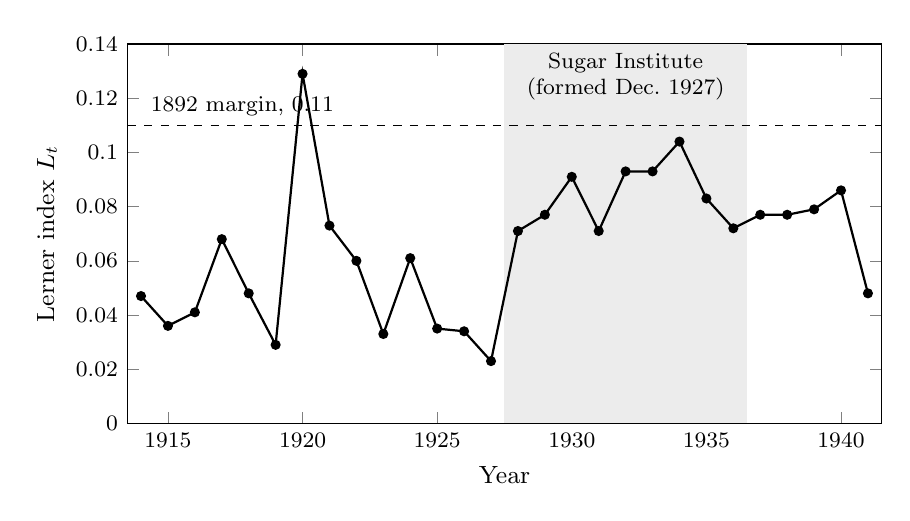
\begin{tikzpicture}
\begin{axis}[
  width=0.92\textwidth, height=6.4cm,
  xmin=1913.5, xmax=1941.5, ymin=0, ymax=0.14,
  xlabel={Year}, ylabel={Lerner index $L_t$},
  xtick={1915,1920,1925,1930,1935,1940},
  x tick label style={/pgf/number format/1000 sep={}},
  ytick={0,0.02,0.04,0.06,0.08,0.10,0.12,0.14},
  y tick label style={/pgf/number format/fixed,/pgf/number format/precision=2},
  tick label style={font=\footnotesize}, label style={font=\small},
  clip=false]
\fill[gray!15] (axis cs:1927.5,0) rectangle (axis cs:1936.5,0.14);
\node[font=\footnotesize, align=center] at (axis cs:1932,0.128) {Sugar Institute\\(formed Dec.\ 1927)};
\draw[dashed] (axis cs:1913.5,0.11) -- (axis cs:1941.5,0.11);
\node[font=\footnotesize, anchor=south west] at (axis cs:1914,0.11) {1892 margin, 0.11};
\addplot[thick, mark=*, mark size=1.4pt] coordinates {
 (1914,0.047) (1915,0.036) (1916,0.041) (1917,0.068) (1918,0.048) (1919,0.029) (1920,0.129)
 (1921,0.073) (1922,0.060) (1923,0.033) (1924,0.061) (1925,0.035) (1926,0.034) (1927,0.023)
 (1928,0.071) (1929,0.077) (1930,0.091) (1931,0.071) (1932,0.093) (1933,0.093) (1934,0.104)
 (1935,0.083) (1936,0.072) (1937,0.077) (1938,0.077) (1939,0.079) (1940,0.086) (1941,0.048)};
\end{axis}
\end{tikzpicture}
\caption{Lerner index of cane sugar refining, 1914--1941, computed from direct marginal cost,
$L_t = \frac{p^{\mathrm{ref}}_t - 1.075\,p^{\mathrm{raw}}_t - 0.60}{p^{\mathrm{ref}}_t}$. The shaded years are
1928--1936. The dashed line is the 1892 margin, which \citet{GenesoveMullin2001} propose as a realistic
monopoly benchmark. Redrawn from \citet{GenesoveMullin2001}, Table~1, column (4).}\label{fig:13-gm-lerner}
\end{figure}

The Lerner index uses list prices, and secret discounts were the reason the Institute was founded. Genesove and
Mullin argue that this bias strengthens their conclusion. The argument takes one line. Let the average
transaction price be $p^{a}_t = p^{\mathrm{ref}}_t - d_t$, where $d_t \ge 0$ is the average secret discount.
Marginal cost is measured directly, so the change in the transaction margin is
\begin{equation}\label{eq:13-gm-lowerbound}
  \Delta\left(p^{a}_t - mc_t\right) = \Delta\left(p^{\mathrm{ref}}_t - mc_t\right) - \Delta d_t
  \;\ge\; \Delta\left(p^{\mathrm{ref}}_t - mc_t\right)
  \quad\text{whenever } \Delta d_t \le 0 .
\end{equation}
If the Institute eliminated secret concessions, or at least did not increase them, the rise in the list margin is
a lower bound on the rise in the transaction margin.

How close did the refiners come to monopoly? The inverse elasticity rule of \cref{sec:02-monopoly} gives a
monopoly Lerner index of $\frac{1}{\varepsilon}$. With the demand elasticity of 1.75 that Genesove and Mullin
estimated for 1890--1914, the monopoly Lerner index is $\frac{1}{1.75} = 0.57$, far above anything in
\cref{tab:13-gm-t1}. The authors give two reasons for the gap. The growth of beet sugar after the First World War
raised the elasticity of demand facing cane refiners, and the refiners wanted to deter foreign and domestic
entry. They propose 11 percent as a realistic benchmark. That was the margin in 1892, when both the margin and
American Sugar Refining's market share (92 percent) reached their peaks. Over 1928--1935 the Lerner index
averaged 0.085 (our computation), about three quarters of that benchmark, as the authors state. The benchmark has
a structural reading. If 0.11 were the Lerner index of a firm pricing optimally against its residual demand, the
inverse elasticity rule would put that residual elasticity at $\frac{1}{0.11} \approx 9$ (our computation). A
perceived elasticity five times the market elasticity is consistent with pricing to limit entry and imports.

Quantities tell the same story more weakly. The output of the Atlantic refiners fell when the Institute began,
though only a little, because sugar demand is inelastic. Output kept falling during the Great Depression, but much
less than the 24 percent fall in total industrial output (p.~382). Rivals outside the agreement expanded. The
share of imported refined sugar, almost all of it Cuban, rose from under half a percent to 6 percent in the
Institute's first year and to almost 15 percent in 1933. The Sugar Act of 1934 then cut it to 11 percent by
legislative fiat. Coca-Cola, the largest buyer of refined sugar, switched entirely to foreign suppliers. The beet
share rose from an average of 15.4 percent in 1924--1927 to 17.7 percent in 1928--1931, but its year-to-year
variability prevents a firm attribution to the Institute.

\casehead{Collusion by rules}
Genesove and Mullin describe the Institute as implicit collusion on price combined with explicit collusion on
business practices (p.~383). Rule number one required ``open prices and publicly announced terms.'' Prices
were posted on the refiners' bulletin boards, the Institute was notified of every change in prices and pricing
methods, and changes were announced by 3:00 p.m. These provisions continued existing practice. The more
important existing practice was the \emph{moves system}. An announced price decrease took effect immediately,
while an increase took effect only after a day. Buyers purchased a month's supply at a time, so they waited after
a decrease until other refiners matched it, which they always did. Reactions often came within minutes. Price
competition therefore preceded trade.

\begin{remark}[Why the moves system leaves only secret deviations]\label{rem:13-moves}
Let $N$ refiners sell a homogeneous good at a common list price $p$ with $c < p \le p^m$, and let industry profit
$\pi(p) = (p - c)D(p)$ be increasing on $[c, p^m]$. Suppose that a public price cut to $p' < p$ is matched by
every rival before any buyer purchases. Buyers then split equally among the refiners, and the cutter earns
$\frac{1}{N}\pi(p')$ in the period. Because $\pi$ is increasing on $[c, p^m]$,
\begin{equation*}
  \frac{1}{N}\,\pi(p') < \frac{1}{N}\,\pi(p) .
\end{equation*}
A public cut lowers the cutter's own profit. Only a concession that rivals cannot see, and hence cannot match,
can raise a refiner's share. This is why the Institute worked to raise the probability of detecting secret
concessions and did not try to shorten reaction times (\citealp{GenesoveMullin2001}, pp.~383--384). The
model of \cref{sec:13-transparency-theory} formalizes this probability.
\end{remark}

Almost every contractual term could hide a price cut, so the rules were wide-ranging and detailed.
\Cref{tab:13-gm-rules} lists the five rules that Genesove and Mullin examine, the concession each one closed, and
the cost it imposed. The Institute also disallowed quantity discounts, allowances for returned sugar bags,
long-term contracts and certain credit arrangements. It required refiners to report all sales of damaged sugar,
drew up a list of permissible consignment points, and forbade downstream firms to combine brokerage and storage.
Enforcing the last rule required private investigation and auditing.

\begin{table}[htbp]
\centering
\caption{Sugar Institute rules, the hidden concessions they closed, and their costs}\label{tab:13-gm-rules}
\small
\begin{tabularx}{\textwidth}{@{}>{\raggedright\arraybackslash}p{2.6cm}>{\raggedright\arraybackslash}X>{\raggedright\arraybackslash}X@{}}
\toprule
Rule & Concession it closed & Cost or side effect\\
\midrule
Water-damaged or frozen sugar & Sound sugar shipped to a favored buyer and invoiced as damaged. Each sale now
required ``full details of amount, location, reason and price'' to be circulated. & Discounts on truly damaged
sugar became public.\\
\addlinespace
Credit terms & Varying the grace period that qualified for the customary 2 percent cash discount. & Grace period
fixed at 7 days rather than 14.\\
\addlinespace
Storage & Brokers who ran warehouses cut storage charges in place of the sugar price. & Storage first banned in
buyers' warehouses, then in broker-affiliated ones as refiners switched.\\
\addlinespace
Delivery time & Letting favored buyers take delivery after the contract date, which saved storage and interest
and was a price cut if the basis price rose. & Delivery dates enforced. Weekly reports of undelivered contracts.
A secondhand market sold overbought sugar at discounts of 5 to 20 cents.\\
\addlinespace
Freight & Rebates on freight rates that the Interstate Commerce Commission did not regulate, especially private
water charters. & Charters registered, uniform rates required, written promises not to rebate. Then delivered
pricing with a refusal to sell f.o.b.\ refinery.\\
\bottomrule
\end{tabularx}

\smallskip
\begin{minipage}{0.95\textwidth}\footnotesize
Notes: Compiled from \citet{GenesoveMullin2001}, Sections II, III and VI (pp.~383--387 and 390--392). The
organization into columns is ours.
\end{minipage}
\end{table}

The rules were costly. A monopolist could have discriminated among customers and exploited efficiencies that the
rules forbade. When large buyers in Buffalo asked to receive sugar by water barge, even at the higher rail rate,
the Institute refused for fear of creating an opportunity for discounts. The move to delivered pricing led
refiners to replace brokers in barge transport. Between 1928 and 1931, barge shipments by refiners rose by 400
percent while those by customers fell by two thirds. Large customers denied quantity discounts threatened to
integrate backward, as the grocery chain A\&P did. The ban on long-term and tolling contracts also sacrificed
efficiencies. Place was even prepared to forgo allocating production by cost. He feared that local differences in
loading costs would lead to different rates, writing that ``those enjoying more economical loading conditions
can pocket the profits.'' The District Court judge put it succinctly (p.~384, fn.~14). The refiners
``preferred to have all sugar sold in any given trade areas at precisely the same prices and terms'' over
economies in distribution.

Genesove and Mullin consider an alternative reading in which the rules suppressed nonprice competition directly.
Contractual harmonization usually chose the lower ``quality.'' The grace period was set at 7 days, and the number
of consignment points was cut by half. They find this reading incomplete for three reasons. It does not explain
many rules, such as the ban on quantity discounts or the notification rules discussed below. The number of sugar
grades was never restricted, although grade proliferation was costly to small refiners. Most persuasively, the
reading misses the stated intermediate goal of eliminating discrimination among customers, the first principle
of the Code of Ethics. They conclude that suppressing nonprice competition complemented harmonization but was
not its purpose.

\casehead{An incomplete agreement and its governance}
The initial agreement was incomplete in the sense of the theory of the firm. No one could foresee and enumerate
all contingencies. The refiners told the court that the Code ``could not be, self-operative'' and required
``interpretation and administration and consultation.'' The weekly meetings completed the contract in three ways.
They answered minor questions the Code left open. May damaged sugar be sold under a price guarantee? No. Do
30-day contracts end on the 30th day or on the same day of the next month? The former. They modified rules that
proved unworkable. The original policy charged the regulated all-rail rate whatever the mode of transport. This
leveraged each refiner's power in its hinterland into contested markets such as the Great Lakes, and cheaper water
routes offered too much arbitrage. A later regime of limited differential rates also failed. The refiners then
moved to delivered prices with a refusal to sell f.o.b.\ refinery. The move was presented as independent action.
The Place memos show that it was coordinated over several meetings in one week of April 1929. It had been delayed
for over a year for fear of the antitrust authorities. Finally, the meetings closed loopholes. Each rule that shut
one channel for secret concessions opened another, less effective one, much as taxpayers respond to a new tax
rule.

The meetings formalized their decisions as Code Interpretations, which took on a quasi-judicial character.
Participants spoke of evidence and precedent. Institute counsel called the Interpretations ``absolutely
indispensable,'' since ``even national laws must be `interpreted' by the Courts.'' Genesove and Mullin argue that
legal principles helped complete the contract. One decision covered many later incidents, disputes were
minimized, and participants could anticipate one another's responses.

A natural worry is that frequent meetings invite renegotiation out of punishments \citep{McCutcheon1997}.
Genesove and Mullin see no sign of it. The refiners chose weekly meetings and no one proposed meeting less often.
Threats were never retracted, and no firm bargained its way out of a punishment (p.~396).

\casehead{Prior notification}
Institute rules required a firm to notify the other members before selling damaged sugar, introducing new private
brands, or changing any terms of trade. Firms also notified one another when no rule required it. Revere, a Boston
refiner, told the Institute before it considered lowering its rail rates to the water rate. Arbuckle announced a
cut in freight rates privately to the members before announcing it publicly. Notification served two purposes.
First, it removed the lag before retaliation in nonprice dimensions, complementing open price announcements. Full
collusion is possible when firms can respond to deviations before consumers act \citep{Bhaskar1989}. In the
language of \cref{sec:13-transparency-theory}, notification makes a nonprice change visible with probability one
before it can steal customers.

Second, notification served the individual interest of the notifying firm. Some actions are profitable once
rivals have responded but steal market share if rivals do not anticipate them. Stealing share risks retaliation.
A Godchaux representative praised Savannah, which explained its need to change its business methods at a Board
meeting before announcing anything. As a result, its ``subsequent announcements, because understood, did not
cause any upheavals.'' Genesove and Mullin describe a two-level agreement. The lower level was a precise set of codes and
resolutions. The higher level was an understanding that a refiner could withdraw from a lower-level rule if it
first told the others. All the cases they record concern an easing of terms of trade. This distinguishes them
from the familiar case of advance notice of price increases, where notice coordinates a move that is profitable
only if all firms follow.

\casehead{Ex post determination of fault}
The meetings were also a forum for accusation and rebuttal. In March 1929, American charged Federal with secretly
cutting prices by loading barges without charge. The dispute turned on what ``f.o.b.'' meant, and Federal
may have believed that other firms loaded barges the same way. As in \citet{GreenPorter1984}, the evidence of
cheating was ambiguous. In their model the confounding factor is a fall in demand. Here it was a
misunderstanding about the terms of the agreement. In other cases it was an
external event, such as a shortage of barges or vacuum pans. An accusation could also be factually wrong. An
Institute investigator once reported a concession on one barrel of caked sugar as a concession on a much larger
amount of powdered sugar.

Genesove and Mullin give two reasons why firms investigated before retaliating. A firm may not have intended to
break the agreement, and the Institute let an accused firm prove its innocence on factual or logical grounds. In
their words, the Institute ``raised the signal-to-noise ratio of indicators of cheating.'' An accuser acting alone
also risked being accused of cheating itself. Evidence that only the accuser could observe was therefore
insufficient, and accusers needed evidence that others could verify. In one case an investigator produced an invoice that seemed to show a sale
from Godchaux to Edgar, a Detroit broker that also ran storage. Place examined the invoice and judged it part of
Godchaux's bookkeeping, and the refiners were notified of ``the error which apparently had been made.''
\Cref{cor:13-false-alarms} below shows why lowering the rate of false accusations relaxes the incentive
constraint.

\casehead{Cheating and retaliation}
In the theory of implicit collusion, every deviation by a player is treated the same way, whatever its nature or
timing. Genesove and Mullin observe something quite different. Firms did cheat. A Detroit chain store received a
secret concession when it switched from National to Spreckels. Spreckels overpaid truckers, who then worked a few
hours ``free'' for certain customers. Arbuckle knowingly sold to a dummy corporation that fronted for Edgar.
Cheating was worst in the South. Godchaux accepted a contract with a price guarantee for delivery by water barge
whose movements it agreed not to trace. Texas City accepted a 42-day contract, and its owner offered to fire his
top three executives over it. Colonial offered a 6-cent rebate to large buyers, and in Tampa postdated checks were
used to give credit (p.~390).

Outside the South, none of these violations led to competitive prices as in \citet{GreenPorter1984}, let alone
to subcompetitive prices as in \citet{AbreuPearceStacchetti1986}. The usual sequence was that fault was
determined, the refiner confessed, justified itself or blamed its broker, and the practice stopped. Longer or open
violations were matched. When one firm openly lowered its rail rate to the barge rate, the others lowered theirs
to the same level. When the Pacific refiners gave a freight allowance, American announced that it would match it.
Matching was in degree and in kind. The response stayed within the instrument of the violation, although
\citet{BernheimWhinston1990} show that punishing across all instruments strengthens collusion. When McCahan
concluded that some refiners were not enforcing contract time limits, Place first threatened, and then with
others carried out, a refusal to enforce McCahan's terms. Matching was even institutionalized. Each refiner
reported its undelivered contracts for each price move, the reports circulated weekly, and an unannounced
understanding let all refiners spread deliveries over as many days as the most delayed refiner.

Massive retaliation came only after large-scale cheating in several dimensions, and only in the South. As early as
June 1929 an investigator reported the Code ``dead in the water'' in Texas. C\&H refused to discuss any single
violation there. It threatened to ask for ``the entire suspension of the Code of Ethics in the Texas territory''
so that all refiners could ``fight fire with fire.'' Elsewhere in the South, Savannah was dissuaded
from resigning by a resolution that allowed members to ``meet the competition of Hershey,'' a Cuban refiner
outside the Institute. The condition was that the competitor and the territory be announced to the Institute
first. The agreement could be suspended, but only with prior notification.

Genesove and Mullin summarize the contrast in terms of statistical errors. In the Green and Porter equilibrium,
firms accept punishing when no one has cheated so that cheating never occurs. The refiners chose the opposite end
of the trade-off. They accepted some cheating so as not to punish inappropriately, and they sustained imperfect
collusion because wholesale cheating did meet massive retaliation. Two features of the industry help explain this
choice. Refiners sold through brokers, who often dealt exclusively with one refiner and earned a fixed commission
on every sale. A broker gained much more from stealing a customer than its refiner did. Brokers' cheating added
noise to demand and let refiners hide behind their brokers. The same agency relation made punishment costly,
since selling agents cannot easily be told to follow one set of rules one day and another the next. Matching also
has a known robustness, as in the ``tit for tat'' strategies of \citet{Axelrod1984}, and it fitted the ethic of
nondiscrimination in the Code.

\casehead{What the refiners did not do}
In the model of \citet{GreenPorter1984} firms monitor a public signal, the market price, and never see their
rivals' outputs (\cref{sec:13-jec-setting}). \citet[p.~90]{GreenPorter1984} note that noisy market-share
information could serve as the signal instead. Genesove and Mullin take this broader reading. They describe
Green-Porter and its offshoots as models in which cheating is inferred from a firm's market share (p.~394). Some
models of imperfect monitoring also transfer share to firms that lost it. Market-share data were available to the
refiners at low frequency, but they rarely used them this way. Genesove and Mullin find only four such incidents in nearly a hundred meetings
over 18 months (p.~394). In one, Arbuckle's low share was blamed on its strict contract enforcement, and the
possibility that American's advertising was responsible was dismissed because others' sales had not fallen. The
reason for a fall in share mattered, unlike in the market-share reading of the theory. There was no mechanism for reallocating market shares.
American twice proposed market-sharing schemes in 1929, but neither came with an enforcement mechanism and
Institute counsel would not allow discussion that ``could bring actual results.'' There were no mergers, and
calls for coordinated market withdrawals went unfulfilled. The contrast with the quota-and-transfer cartels of
\citet{HarringtonSkrzypacz2011}, discussed in \cref{sec:13-imperfect}, is sharp.

\casehead{Interpretation, critiques and contribution}
The Institute did more than host communication. It was a neutral party that could audit members and aggregate
self-reported statistics into confidential industry totals. Firms could also use it as a scapegoat or a
commitment device in bargaining with brokers and buyers. Genesove and Mullin draw three lessons for theory.
Collusive agreements are incomplete and need governance. Communication within the agreement is rich, with prior
notification and ex post determination of fault. Retaliation is much more restrained than theory predicts,
partly because of selling agents' high-powered incentives. They also stress that Stigler's basic insight
survives. The rules were built by firms that knew each would later want to undermine them.

The evidence has limits. The notes come from one participant at a midsize refinery and cover 18 months of a
nine-year cartel. The performance measures use list prices. A list price is never below the transaction price, so the list
margin bounds the level of the transaction margin from above. Only the rise in the transaction margin is bounded
from below, by the rise in the list margin, and \eqref{eq:13-gm-lowerbound} gives that bound only if secret
discounts did not grow. There is no counterfactual for what prices would have been without the
Institute in the Great Depression, and the rise in imports shows that the cartel's market power was limited.
Inferring strategies from what participants said requires trusting that they described their reasoning
accurately, a premise the authors defend. The forgone efficiencies are public, while those in
\citet{AtheyBagwellSanchirico2004} are private information, so that theory cannot explain why the refiners gave
them up. Genesove and Mullin's own explanation is that exploiting the efficiencies would have destroyed the
homogeneity of practices that made pricing transparent. The paper's contribution is to show that cartels can
invest in detection itself, through rules that make contracts comparable and through a forum that judges
evidence. It also poses the puzzle of tolerated cheating that \citet{BernheimMadsen2017} later addressed
(\cref{sec:13-imperfect}).

\subsection{Price wars in pre-1914 sugar refining}\label{sec:13-gm-pricewars}

The same industry provides a test of what price and cost data can say about conduct. \Cref{sec:03-sugar-wars}
analyzes the two post-entry price wars of 1890--1914 studied by \citet{GenesoveMullin1998}. They followed the
entry of Spreckels (January 1890 to February 1892) and of Arbuckle and Doscher (September 1898 to April 1900).
Conduct is $\theta_t = \theta_0 + (\theta_1 - \theta_0)\mathit{WAR}_t$. Direct cost data give
$\theta_0 = 0.129$ and $\theta_1 - \theta_0 = -0.127$ in the published article \citep[Table~10]{GenesoveMullin1998},
so conduct in the wars
was $0.002$, essentially competitive. The NBER working paper on file reports 0.11 and $-0.09$ for the same direct
measures (\citealp{GenesoveMullin1995}, Table~14, column~(9)). Holding marginal cost fixed across regimes, the
nonlinear instrumental-variables estimates detect the fall. With linear demand, $\hat\theta_1 - \hat\theta_0 =
-0.112$ (0.069) when $k$ is estimated and $-0.108$ (0.051) when $k = 1.075$ is imposed (\cref{tab:03-gm-pricewars},
Panel A). These two estimates are the same in both versions (working paper, Table~14, columns~(3) and~(4)).

When the cost intercept may also shift in the wars, the same estimator attributes the wars to falling cost. The
estimated cost drop is 10 to 18 cents per hundred pounds and the fall in conduct only 0.015 to 0.024 across
demand forms (\citealp{GenesoveMullin1995}, Table~15). Neither difference is significant. This is
\cref{prop:13-obs-equiv} in real data. Prices and quantities alone cannot separate a switch in conduct from a
switch in cost. Prior information that costs were stable, available here from the technology, breaks the tie.
The Sugar Institute era of \cref{sec:13-sugar-institute} is the same industry a generation later, when the
refiners tried to avoid such wars by rules rather than by punishment.

\subsection{The bromine cartel, 1885--1914}\label{sec:13-bromine}

\casehead{The question}
Why do cartels fight price wars? In \citet{GreenPorter1984} and \citet{AbreuPearceStacchetti1986} (APS
hereafter), price wars are equilibrium punishments. Firms cannot see one another's actions, so they punish after
unfavorable public signals even though no one cheats (\cref{ch:collusion-theory}). An older view, associated with
\citet{Stigler1964}, sees price wars as breakdowns caused by cheating or entry. \citet{Levenstein1997} uses
internal documents of the bromine industry, including contracts, correspondence and minutes of negotiations, to
ask which view fits. She finds that both do, for different wars. Short, mild wars came from imperfect
information. Long, severe wars were part of bargaining over the division of rents.

\casehead{The industry}
Bromine was first produced commercially in 1845. During the Civil War, army medics discovered the sedative
properties of potassium bromide, which became a popular patent medicine for headaches and nervous disorders. In
Europe bromine was used in aniline dyes, but this use was negligible in the United States until after the First
World War. Before 1892 a dozen small firms near the Ohio River, in southeast Ohio and northwest West Virginia,
produced all U.S.\ bromine by pumping and heating underground brine. They sold liquid bromine to
\emph{manufacturing chemists}, larger urban firms that converted it into potassium bromide powder and distributed
it to pharmacies. The two most important were Powers \& Weightman (P\&W) and Mallinckrodt Chemical Works. The only
other significant producers were German potash mines. They belonged to a bromine cartel allied with the German
potash cartel, which had the active support of the German state.

\casehead{The cartel's organization}
Collusive institutions controlled the market for most of 1885--1914, and their form changed three times
(\cref{fig:13-lev-contracts}). In 1885 the National Bromine Company (NBC) contracted with the Ohio River firms to
buy their entire output for five years at a specified price. The contracts forbade sales to anyone else.
Mallinckrodt and P\&W in turn agreed to buy all of the NBC's bromine, and they announced the price of potassium
bromide in coordination. That price rose from 26.5 cents per pound at the end of 1884 to 34 cents right after the
contracts were signed in March 1885. The NBC expired in March 1891. A new pool was not formed until October 1892.
W.~R. Shields of Columbus, Ohio then contracted with each producer to buy its entire output for five years, and he
sold it to Mallinckrodt and P\&W. These two firms agreed with the German cartel not to export, and the Germans
agreed to buy \$25,000 of bromine a year from them.

Herbert Dow's entry changed the industry. His Midland Chemical Company, incorporated in 1892 and merged with the
Dow Chemical Company in 1900, used an electrolytic process. It produced bromine and bromide salts continuously
and more cheaply, and its minimum efficient scale was at least ten times that of an Ohio River producer. Dow never
joined the pool but sold its entire output to Mallinckrodt and P\&W under a one-year contract in 1894. The
contract limited Midland's output and forbade other sales. Two more one-year contracts followed, then a five-year
contract in 1897. In the spring of 1902 Dow ended its cooperation and signed with two rival chemists, Rosengarten
\& Sons and George Merck \& Company. Shields' contracts expired in October 1902 and were not renewed.

\begin{figure}[htbp]
\centering
\tikzset{lbox/.style={draw, rounded corners=1pt, align=center, inner sep=2pt, font=\scriptsize},
         lcart/.style={lbox, fill=gray!25}}
\begin{subfigure}[b]{0.32\textwidth}\centering
\begin{tikzpicture}[>=Stealth]
\node[lbox] (ohio) at (0,3.1) {Ohio River producers\\(about 12)};
\node[lcart] (nbc) at (0,2.0) {National Bromine\\Company};
\node[lcart] (mal) at (-0.95,0.9) {Mallinckrodt};
\node[lcart] (pw) at (0.95,0.9) {P\&W};
\node[lbox] (ph) at (0,-0.15) {Retail pharmacists};
\draw[->] (ohio) -- (nbc);
\draw[->] (nbc) -- (mal); \draw[->] (nbc) -- (pw);
\draw[->] (mal) -- (ph); \draw[->] (pw) -- (ph);
\end{tikzpicture}
\caption{NBC pool, 1885--1891}
\end{subfigure}\hfill
\begin{subfigure}[b]{0.32\textwidth}\centering
\begin{tikzpicture}[>=Stealth]
\node[lbox] (ohio) at (-0.9,3.1) {Ohio River\\producers};
\node[lbox] (dow) at (1.05,3.1) {Midland/\\Dow};
\node[lcart] (sh) at (-0.9,2.0) {Shields};
\node[lcart] (mal) at (-0.95,0.9) {Mallinckrodt};
\node[lcart] (pw) at (0.95,0.9) {P\&W};
\node[lbox] (ph) at (0,-0.15) {Retail pharmacists};
\draw[->] (ohio) -- (sh);
\draw[->] (sh) -- (mal); \draw[->] (sh) -- (pw);
\draw[->] (dow) -- (mal); \draw[->] (dow) -- (pw);
\draw[->] (mal) -- (ph); \draw[->] (pw) -- (ph);
\end{tikzpicture}
\caption{Shields pool, 1892--1902}
\end{subfigure}\hfill
\begin{subfigure}[b]{0.32\textwidth}\centering
\begin{tikzpicture}[>=Stealth]
\node[lbox] (ohio) at (-0.45,3.1) {Ohio River\\producers};
\node[lcart] (dow) at (-0.45,2.0) {Dow Chemical};
\node[lbox] (oth) at (1.45,2.0) {Other\\non-retail\\customers};
\node[lcart] (mal) at (-1.35,0.9) {Mallinckrodt};
\node[lcart] (pw) at (0.0,0.9) {P\&W};
\node[lcart] (me) at (1.2,0.9) {Merck};
\node[lbox] (ph) at (0,-0.15) {Retail pharmacists};
\draw[->] (ohio) -- (dow);
\draw[->] (dow) -- (oth);
\draw[->] (dow) -- (mal); \draw[->] (dow) -- (pw); \draw[->] (dow) -- (me);
\draw[->] (mal) -- (ph); \draw[->] (pw) -- (ph); \draw[->] (me) -- (ph);
\end{tikzpicture}
\caption{After 1910}
\end{subfigure}
\caption{Contractual relationships in the bromine industry. Arrows show the flow of bromine under the
contracts. Shaded boxes reproduce the filled boxes of the original figures, which mark the firms at the center of
each arrangement. In panel (c), P\&W is Powers-Weightman-Rosengarten, as Dow's 1908 contracts name it. Redrawn from
\citet{Levenstein1997}, Figures~2--4.}\label{fig:13-lev-contracts}
\end{figure}

International relations followed a similar path. In September 1902 Dow and the German bromine combine agreed in
writing that neither would export potassium bromide to the other's home market. Dow confirmed the agreement and
soon began exporting to Europe in secret. In 1905 the Germans abrogated their side and entered the U.S.\ market.
A detailed agreement at the end of 1908 ended the resulting war. Dow and the Germans set prices jointly in the
United States, Europe and the rest of the world. Dow withdrew from Europe for a payment of \$32,000 a year and
received a one-third share of sales in the rest of the world, and the Germans withdrew from North America. Dow
also signed ten-year contracts to supply all the bromine needs of three manufacturing chemists. It kept the price
of potassium bromide below 20 cents for a year and a half, a price at which the Ohio River firms could not sell
profitably. In May 1910 it contracted to buy the entire output of all but one of them on a sliding scale tied to
the published price. Prices then rose slowly but steadily until the First World War.

\casehead{Evidence of success}
The firms' account books have not survived, so Levenstein assembles indirect evidence. Midland paid its first
dividend after its 1894 contract, followed by regular monthly dividends of two to five percent, when annual
interest rates in the region averaged less than 6.5 percent. Dow, Shields, Mallinckrodt and the Germans made
trans-Atlantic trips for no purpose other than negotiating collusive agreements. Shields supported his family for
a decade on the rents he kept for organizing the pool.

Prices give stronger evidence. The price of bromine fell from six dollars a pound before the Civil War to 30
cents in 1875. It fell another 7 percent by 1880 and almost 30 percent more by 1884. The NBC reversed the trend. The average price of potassium bromide during the NBC pool, 34.08 cents, was almost 10 percent above
the 31.07 cents of the preceding five years. When the NBC contracts ended in 1891, prices fell by almost 30
percent. The Shields pool averaged 40.88 cents, 65 percent above the 24.75 cents between the two pools (the paper
says 60 percent) and 31.6
percent above the prices of 1880--1885. When the Shields contracts expired in 1902, the price fell 43.2 percent
in one month. Between 1902 and 1914, the average price was 29.3 cents during cooperation and 16.8 cents
otherwise, almost 75 percent higher. The price jumped from 13 to 19 cents on December 21, 1908, the day the Dow
and German agreement took effect. The same comparisons hold for prices deflated by a wholesale chemical price
index. For example, real prices after 1902 were 74 percent higher during cooperation (WP pp.~9--11, fns.~19--23).

Costs confirm that prices exceeded marginal cost. Dow estimated the marginal cost of a pound of bromine under the
Ohio River process at 12 cents. Shields paid the Ohio River producers 16 cents in the first year of his contracts,
rising by 2 cents a year to 22 cents. For potassium bromide, Levenstein estimates the cost of manufacture as
\begin{equation}\label{eq:13-lev-cost}
  TC(Q) = Q\left(0.85\,P_{\mathrm{Br}} + 0.6\,P_{\mathrm{KOH}} + C_{\mathrm{mc}}\right).
\end{equation}
Here $P_{\mathrm{Br}}$ is the contract price of bromine and $P_{\mathrm{KOH}}$ the market price of potash. The
term $C_{\mathrm{mc}} = 4$ cents is the chemists' processing and distribution cost per pound. During the Shields pool the
price averaged 40.9 cents and this cost 24.1 cents, a markup of almost 70 percent (WP Figure~5). The correlation
between changes in price and changes in cost was $-0.042$. Dow's own cost of potassium bromide was about 8 cents
before 1902, while its 1897--1902 contract paid 25 cents. Prices were also more stable under cooperation.
They changed on average every 41.1 weeks during cooperation and every 11.5 weeks otherwise. Within the pool years
the figures were 35 and 6.8 weeks, and after 1902 they were 64.7 and 17.5 weeks. Many firms announcing prices
independently raise the chance that some price changes in a given week.

\casehead{How close to monopoly}
Levenstein compares the pool price with the prices that monopoly, Cournot and perfect competition would produce.
She considers three linear inverse demand curves for potassium bromide. Each is consistent with aggregate data
and is fitted through the average prices and outputs of two years:
\begin{equation}\label{eq:13-lev-demand}
  \text{I: } P = 78 - 0.077\,Q, \qquad
  \text{II: } P = 67 - 0.038\,Q, \qquad
  \text{III: } P = 173 - 0.203\,Q .
\end{equation}
Prices $P$ are in cents per pound and quantities $Q$ in thousands of pounds a year. Demand I uses 1895 and 1909, II uses 1896 and
1908, and III uses 1897 and 1909. Each firm's cost is \eqref{eq:13-lev-cost} plus a fixed cost, evaluated at
$P_{\mathrm{Br}} = 12$ (Dow's marginal cost estimate) and $P_{\mathrm{KOH}} = 4$ (the average potash price in the
pool period). Marginal cost is therefore constant at
\begin{equation}\label{eq:13-lev-mc}
  c = 0.85 \times 12 + 0.6 \times 4 + 4 = 10.2 + 2.4 + 4 = 16.6 \text{ cents.}
\end{equation}

\begin{example}[Reproducing Levenstein's Table~2]\label{ex:13-lev-cournot}
Let inverse demand be $P = a - bQ$ and let $N$ firms have constant marginal cost $c$. Firm $i$ maximizes
$(a - bQ - c)q_i$. Its first-order condition is
\begin{equation*}
  a - bQ - c - b\,q_i = 0 .
\end{equation*}
In a symmetric equilibrium $q_i = \frac{Q}{N}$. Substituting,
\begin{equation*}
  a - c = bQ\left(1 + \frac{1}{N}\right)
  \quad\Longrightarrow\quad
  Q = \frac{N}{N+1}\,\frac{a - c}{b}, \qquad
  P = a - bQ = \frac{a + Nc}{N+1}.
\end{equation*}
For Demand I, $\frac{a - c}{b} = \frac{78 - 16.6}{0.077} = 797.4$ thousand pounds, the competitive output.
Monopoly ($N = 1$) gives $Q = 398.7$ and $P = \frac{78 + 16.6}{2} = 47.3$ cents. Duopoly gives $Q = 531.6$ and
$P = \frac{78 + 33.2}{3} = 37.1$. Twelve firms, about the number active in 1891, give $Q = 736.1$ and
$P = \frac{78 + 199.2}{13} = 21.3$. Competition gives $P = c = 16.6$. These are exactly the entries of
\cref{tab:13-lev-t2}.
\end{example}

\begin{table}[htbp]
\centering
\caption{Monopoly, Cournot and competitive outcomes for potassium bromide}\label{tab:13-lev-t2}
\small
\begin{tabular}{@{}lccccc@{}}
\toprule
 & \multicolumn{3}{c}{Demand I} & Demand II & Demand III\\
\cmidrule(lr){2-4}\cmidrule(lr){5-5}\cmidrule(l){6-6}
Number of firms & $q_i$ & $Q$ & $P$ & $P$ & $P$\\
\midrule
1 (joint maximum) & 398.7 & 398.7 & 47.3 & 41.8 & 94.8\\
2 & 265.8 & 531.6 & 37.1 & 33.4 & 68.7\\
12 & 61.3 & 736.1 & 21.3 & 20.5 & 23.6\\
$\infty$ & & 797.4 & 16.6 & 16.6 & 16.6\\
\midrule
\multicolumn{6}{@{}l}{Pool average price, 1885--1902, excluding price wars: 38.6 cents}\\
\bottomrule
\end{tabular}

\smallskip
\begin{minipage}{0.92\textwidth}\footnotesize
Notes: Reproduced from \citet{Levenstein1997}, NBER working-paper version, Table~2. Quantities in
thousands of pounds a year, prices in cents per pound. Demand functions in \eqref{eq:13-lev-demand}, marginal
cost 16.6 cents from \eqref{eq:13-lev-mc}. The Demand III entry for 12 firms is printed as 23.6. The printed
quantity of 711.2 and the formula of \cref{ex:13-lev-cournot} both give $P = \frac{173 + 199.2}{13} = 28.6$
(our computation), so 23.6 appears to be a misprint.
\end{minipage}
\end{table}

The pool average of 38.6 cents lies between the twelve-firm Cournot price of 21.3 and the monopoly price of 47.3
under Demand I. Levenstein concludes that the pool raised prices above competitive and usually above Cournot
levels, without reaching monopoly. Collusive prices ranged from 19 to 46 cents. The conduct parameter of
\cref{sec:02-conduct} summarizes the pool price in one number. With linear demand the supply relation is
$P = c + \theta bQ$, so $bQ = \frac{a - c}{1 + \theta}$ and $P = \frac{\theta a + c}{1 + \theta}$. Solving for
$\theta$ at the pool price gives
\begin{equation*}
  \theta = \frac{P - c}{a - P} = \frac{38.6 - 16.6}{78 - 38.6} = \frac{22.0}{39.4} = 0.56
\end{equation*}
(our computation). This lies between symmetric Cournot duopoly ($\theta = \frac{1}{2}$) and joint profit
maximization ($\theta = 1$).

Levenstein also measures the welfare cost of the pool. At 38.6 cents, Demand I gives an output of
$\frac{78 - 38.6}{0.077} = 511.7$ thousand pounds and revenue of \$197,500 (our computation), matching the
\$197,516 she reports. She reports a deadweight loss of \$44,568 a year, less than six
hundredths of a cent per person in 1900. The loss is about 23 percent of industry revenue (our computation), although
the paper says about 25 percent. The triangle between Demand I and the marginal cost of
\eqref{eq:13-lev-mc} is smaller. It equals $\frac{1}{2}(38.6 - 16.6)(797.4 - 511.7) = 3{,}143$ thousand
cent-pounds, or about \$31,400 (our computation).\footnote{Her figure is matched by a marginal cost of about 12.4
cents (our computation). The paper does not state which cost benchmark the deadweight loss uses.}

\casehead{Testing the order of the regime process}
Green and Porter's trigger strategies imply wars of fixed length $T-1$, so the regime process is Markov of order
$T-1$. In APS the length of a war is random and the regime follows a first-order Markov process. Levenstein applies
the test of \citet{BerryBriggs1988}, described in \cref{sec:13-tests}, to two regime series for 1885--1914, one
weekly and one monthly. Each series sets $I_t = 1$ when the firms collude and $I_t = 0$ otherwise. The series
come from reports of collusive activity in the \textit{Oil, Paint and Drug Reporter} and from Dow's papers, and
prices were not used to build them. She did not estimate regimes by switching regressions, as \citet{Porter1983}
did. Demand shifted with regime changes because buyers speculated on whether a break in prices would last, so
the supply relation was not stable across regimes (WP p.~16, fn.~35).

The statistic is $W$ of \eqref{eq:13-bb-test}, which compares the conditional frequencies $\hat p_h$ across
histories $h$ that share the same last period. With a single restriction it reduces to a squared $t$-statistic for
the difference of two frequencies. In the monthly two-period test, the histories $(I_{t-2}, I_{t-1}) = (0,0)$ and
$(1,0)$ have $\hat p = 0.068$ with $N = 73$ and $\hat p = 0.167$ with $N = 6$. (Levenstein's tables list histories
in the order $(t-1, t-2)$.) The statistic for their equality is
\begin{equation*}
  W = \frac{(0.068 - 0.167)^2}{\frac{0.068 \times 0.932}{73} + \frac{0.167 \times 0.833}{6}}
    = \frac{0.00980}{0.00087 + 0.02318} = 0.408 ,
\end{equation*}
which reproduces her Table~3 (our computation). Levenstein treats a restriction as untestable when one of its cells
has $\hat p_h \in \{0, 1\}$, and hence zero estimated variance (WP p.~17). She drops such restrictions. In the
monthly series this leaves one restriction, hence one degree of freedom. In the weekly series every restriction
involves a degenerate cell, so she reports no statistic. For those cells she computes instead the probability, under
the first-order null, of the run that occurred. For example, six continued weeks of collusion after a collusive
week have probability $0.994^{6} = 0.965$ when the continuation probability is 0.994. No such probability falls
below 0.68.

\begin{table}[htbp]
\centering
\caption{The regime process of the bromine cartel}\label{tab:13-lev-markov}
\small
\begin{tabular}{@{}lcc@{}}
\toprule
 & Weekly series & Monthly series\\
\midrule
\multicolumn{3}{@{}l}{\textit{Panel A. Transition probabilities (Table 5)}}\\
$\Pr(I_t = 1 \mid I_{t-1} = 1)$ & 0.995 & 0.978\\
\quad periods with $I_{t-1} = 1$ & 1{,}195 & 275\\
$\Pr(I_t = 1 \mid I_{t-1} = 0)$ & 0.017 & 0.076\\
\quad periods with $I_{t-1} = 0$ & 394 & 79\\
$W$ for history independence, 1 df & 18{,}139.1 & 844.0\\
Implied mean collusive spell (our computation) & 200 weeks & 45.5 months\\
Implied mean price war (our computation) & 58.8 weeks & 13.2 months\\
\addlinespace
\multicolumn{3}{@{}l}{\textit{Panel B. First order against higher order (Tables 3 and 4)}}\\
Two-period alternative, $W$ (p-value) & not computable & 0.408 (0.52)\\
Three-period alternative, $W$ (p-value) & not computable & 0.358 (0.55)\\
\addlinespace
\multicolumn{3}{@{}l}{\textit{Panel C. Kolmogorov-Smirnov test of war durations (Table 6)}}\\
Statistic $d_6$ & 0.352 & 0.340\\
Rejection threshold at the 20 percent level & 0.41 & 0.41\\
\bottomrule
\end{tabular}

\smallskip
\begin{minipage}{0.88\textwidth}\footnotesize
Notes: From \citet{Levenstein1997}, NBER working-paper version, Tables~3--6. Levenstein drops every restriction
that involves a cell with zero estimated variance. In the weekly series every restriction does, so the weekly two-
and three-period tests are not computable. Levenstein reports
``significance'' levels of 0.477 and 0.450, which are one minus the p-values shown. Mean spells use
\cref{lem:13-durations}, for example $\frac{1}{1 - 0.995} = 200$ and $\frac{1}{0.017} = 58.8$.
\end{minipage}
\end{table}

\Cref{tab:13-lev-markov} collects the results. First order cannot be rejected against two- or three-period
alternatives, with p-values of 0.52 and 0.55. History independence is rejected overwhelmingly against a
one-period alternative. A second test compares the distribution of war durations with the geometric distribution
implied by a first-order process. With the weekly exit probability 0.017, the probability that a war has ended
within $t$ weeks is $F(t) = 1 - (1 - 0.017)^t$. The six wars lasted 6, 12, 21, 22, 82 and 201 weeks. The
Kolmogorov-Smirnov statistic is the largest gap between this $F$ and the empirical distribution. It occurs at
$t = 22$, where four of six wars have ended,
\begin{equation*}
  d_6 = \frac{4}{6} - \left[1 - (0.983)^{22}\right] = 0.667 - 0.314 = 0.352
\end{equation*}
(our computation reproduces her statistic). This is below the 20 percent threshold of 0.41, so the first-order
model is not rejected. The mean of the six durations, 57.3 weeks, is close to the predicted 58.8 weeks.

These tests have little power. Six wars cannot distinguish a geometric distribution from many alternatives, and
the mean duration is driven by one war of 201 weeks. A geometric distribution with mean 58.8 weeks has a median
of about 40 weeks, against an observed median of 21.5 weeks (our computation). Levenstein's conclusion from the
statistics is modest. Like \citet{BerryBriggs1988} for the Joint Executive Committee, she finds the bromine
regimes closer to APS than to Green and Porter. The historical record then raises serious doubts about both.

\casehead{The six price wars}
The trade press announced six price wars, three before Dow's entry and three after it. \Cref{tab:13-lev-t7}
reproduces Levenstein's comparison. An optimal APS punishment is the same after any history, prescribes the same
behavior in every punishment period, and is the worst equilibrium punishment. None of these holds. The initial
drop ranged from 0 to 15 cents, or 0 to 50 percent (1 to 15 cents in the five wars with an initial drop). Prices stayed flat in the first two wars but spiralled down
for 73 and 149 weeks in Pool III and Dow III. The lowest prices ranged from 32.5 to 13 cents. Only Pool III and
Dow III reached the one-shot Cournot level of \cref{tab:13-lev-t2}, and no war pushed price below marginal
cost.\footnote{In Dow III the price fell to 13 cents, below the twelve-firm Cournot prices of
\cref{tab:13-lev-t2}. By 1905 Dow produced more than half of U.S.\ output at a marginal cost below 10 cents, so
the table's Ohio River costs no longer applied (WP fns.~38--39).}

\begin{table}[htbp]
\centering
\caption{Characteristics of the bromine price wars}\label{tab:13-lev-t7}
\small
\setlength{\tabcolsep}{4pt}
\begin{tabularx}{\textwidth}{@{}>{\raggedright\arraybackslash}p{2.2cm}*{6}{>{\centering\arraybackslash}X}@{}}
\toprule
 & Pool I & Pool II & Pool III & Dow I & Dow II & Dow III\\
 & 1886--1887 & 1888 & 1891--1892 & 1902 & 1903 & 1905--1908\\
\midrule
Initial drop (cents) & 2 & 1.5 & 1 & 4 & 0 & 15\\
Initial drop (\%) & 6.0 & 4.4 & 3.0 & 9.1 & 0 & 50\\
Total drop (cents) & 2 & 1.5 & 13 & 19 & 0 & 17\\
Total drop (\%) & 6.0 & 4.4 & 39.4 & 43.2 & 0 & 56.7\\
Duration (weeks) & 22 & 12 & 82 & 6 & 21 & 201\\
Weeks to trough & 1 & 1 & 73 & 6 & 0 & 149\\
Low price (cents) & 32 & 32.5 & 20 & 25 & 25 & 13\\
\addlinespace
Initial cause & Germans cut price to force U.S.\ firms out of Europe & Germans believe U.S.\ firms export to
Europe & NBC expires, dispute over new pool terms & Dow signs with non-pool distributors & Dow tries to raise
price, pool distributors refuse & Germans respond to Dow's entry into Europe\\
\addlinespace
Central cause & Coordination & Information & Coordination & Both & Unclear & Both\\
\bottomrule
\end{tabularx}

\smallskip
\begin{minipage}{0.95\textwidth}\footnotesize
Notes: Reproduced from \citet{Levenstein1997}, NBER working-paper version, Table~7. All prices are
for potassium bromide from the \textit{Oil, Paint and Drug Reporter}. Price-war periods were determined from
reports in that journal and internal documents, independently of prices. ``Unclear'' renders the table's
question mark.
\end{minipage}
\end{table}

\casehead{Two kinds of price war}
Levenstein attributes the differences to different causes. Pool War~II and Dow War~I came from imperfect
information. In 1888 the Germans saw bromides imported into their markets and took them as a sign that
Mallinckrodt and P\&W had exported in violation of their agreement. It is not clear whether the Germans were
mistaken or whether customers outside the agreement resold bromine. In 1902 Mallinckrodt and P\&W read Dow's
contracts with Rosengarten and Merck as a sign that Dow would undercut the pool. They cut their price as soon as the
Shields contracts expired. Both wars were short and ended after an exchange of letters reaffirming the commitment
not to compete on price. After Dow War~I the firms adopted a new device, pricing at the price announced in the
\textit{Oil, Paint and Drug Reporter}, to prevent further misunderstandings. Neither war took prices to Cournot
levels.

Levenstein explains why these wars were mild. More severe punishments would not have been renegotiation-proof.
Members discounted threats to price below marginal cost. Dow's executives assessed the credibility of each threat
and demanded verification of the inventories that Mallinckrodt and P\&W claimed to hold. Threats nonetheless
mattered. In December 1892 Shields wrote to Dow that his contracts gave him the right to annul them ``should a new
producer of bromine appear.'' Midland then agreed to restrict its output and sell only to Mallinckrodt and P\&W.
Between 1894 and 1896 Midland's quota rose from 150,000 to 200,000 pounds a year, while its capacity exceeded
350,000 pounds. Midland accepted a five-year contract limiting it to 200,000 pounds in 1897. It accepted
largely because it believed the chemists held 800,000 pounds of bromine, which they threatened to sell if Midland
did not cooperate.

Pool War~III and Dow War~III were different. They were prolonged by information problems, such as the Germans'
ignorance of Dow's costs, but did not result from them. Firms publicly announced that they would sell below the
old collusive price, and everyone understood the announcements as moves in a renegotiation of the division of
rents. In Dow War~III the Germans offered bromides in New York at 15 cents, half the market price. Dow withdrew
from the U.S.\ market and sold its entire output abroad, a response the Germans had not anticipated. The war
lasted until prices reached all-time lows and Dow's representatives had made three trans-Atlantic trips. Dow
learned the German ``Queensbury rules'' of commercial warfare during the negotiations. One rule gave ``the firm that
shows their ability to get the market in a fight'' the same share in the next truce (WP p.~24). With shares in the next truce tied to shares during the war, prices spiralled down. In
these wars the price war itself shaped the next collusive equilibrium. It was not a punishment that restored the
old one.

\casehead{Learning to avoid price wars}
The 1908 agreement between Dow and the Germans included price-war punishments, but they were never used. When
cheating was suspected, the parties identified the most likely culprit, sometimes by chemical analysis of the
bromide. The culprit then made a cash side payment based on a low estimate of its gain. Such firm-specific
transfers sustain more profitable equilibria than common price wars when outcomes reveal who deviated
\citep{AbreuPearceStacchetti1990,FudenbergLevineMaskin1994}. Levenstein offers two reasons for the change. The
firms learned, having started from the price-war punishments common in other pools of the period. The number of
parties also fell and their identities stabilized, which made it easier to identify a cheater and more worthwhile
to invest in information. Genesove and Mullin cite the tit-for-tat clause in the Dow and German agreement as a
parallel to the Sugar Institute's matching. The transfers anticipate those of \citet{HarringtonSkrzypacz2011}.

\begin{figure}[htbp]
\centering
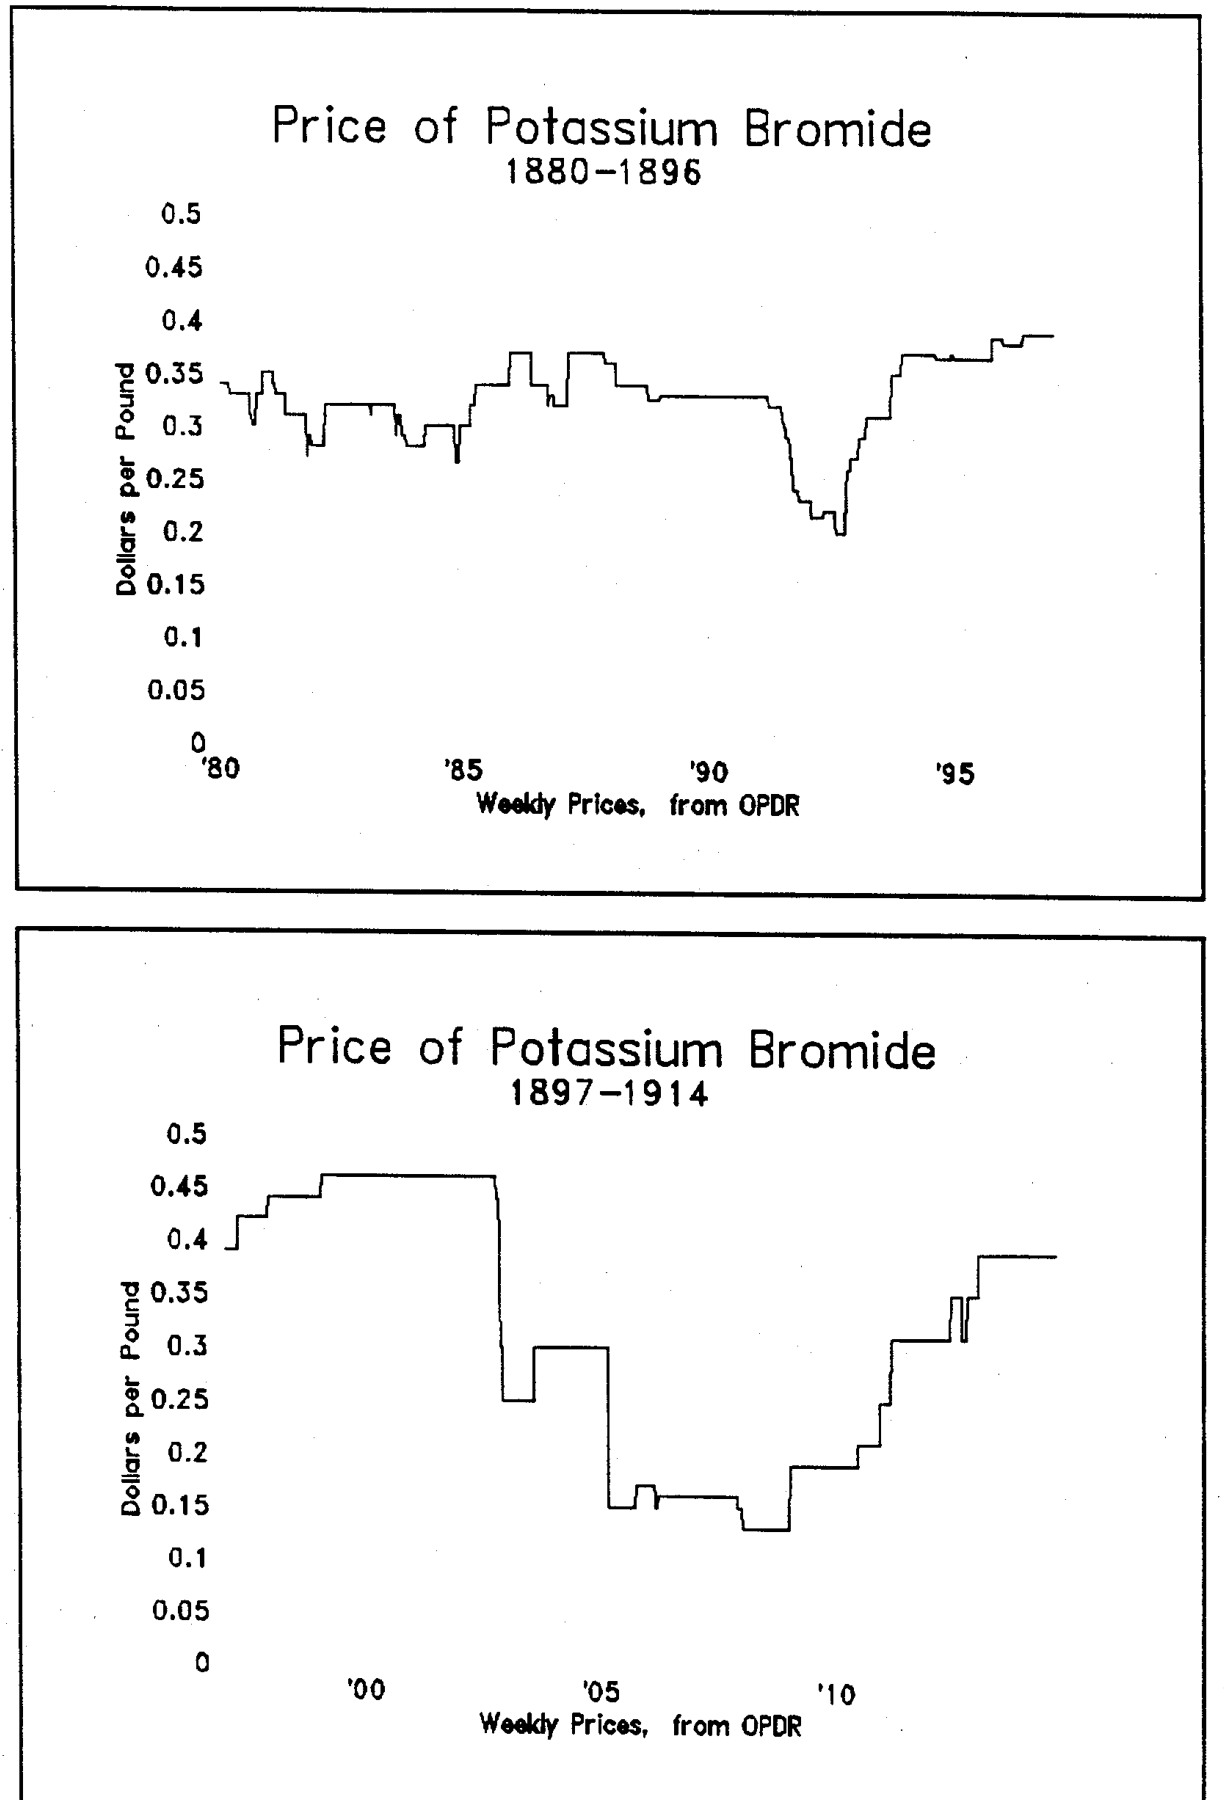
\includegraphics[width=0.62\textwidth]{figures/ch13/levenstein1997_fig1.png}
\caption{Weekly price of potassium bromide in dollars per pound, 1880--1896 (top) and 1897--1914 (bottom), from
the \textit{Oil, Paint and Drug Reporter}. The drop of 1891--1892 is Pool War~III, the collapse of 1902 is Dow
War~I, and the long trough of 1905--1908 is Dow War~III. Source: \citet{Levenstein1997}, Figure~1 (NBER
working-paper version).}\label{fig:13-lev-price}
\end{figure}

\casehead{Assessment}
\Cref{fig:13-lev-price} shows the episodes. The study's strength is its sources. The regime series and the
causes of each war come from documents written by the participants, independently of prices. Its quantitative
parts are weaker. Each demand curve is fitted through two years of aggregate data. Costs come from Dow's estimates
of Ohio River costs, and the deadweight-loss figure cannot be reproduced from the stated cost. The statistical
tests rest on six wars. The paper's contribution is conceptual. Some price wars fit equilibrium punishment under
imperfect monitoring, but they were mild because severe punishments are not credible. Other price wars were
bargaining over the terms of the next agreement, and their severity reflected the stakes of that bargaining.

\section{Information, Transparency and Coordination}\label{sec:13-information}

The Sugar Institute shows firms investing in the detection of secret price cuts. This section asks the same
question from the policy side. What happens when an outside body makes prices more transparent, or when firms use
an information system to signal intentions? We first derive the basic theoretical result, which formalizes
\citet{Stigler1964}. We then study three cases. Danish authorities published firm-specific concrete prices and
prices rose \citep{AlbaekMollgaardOvergaard1997}. The U.S.\ Department of Justice restricted how airlines could
communicate through their fare-publishing system, with temporary effects \citep{Miller2010}. Universities agreed
on financial aid formulas, and their average prices did not change \citep{CarltonBambergerEpstein1995}.

\subsection{Transparency and the incentive constraint}\label{sec:13-transparency-theory}

We embed imperfect detection in the Bertrand supergame of \cref{ch:collusion-theory}. The detection probability
is a reduced-form summary of everything that lets firms infer secret price cuts, such as their own sales, the
trade press, published prices or audits.

\begin{assumption}[Bertrand supergame with imperfect detection]\label{asm:13-transparency}
\leavevmode
\begin{enumerate}[label=(\roman*)]
\item There are $N \ge 2$ firms selling a homogeneous good at constant marginal cost $c$. Industry profit
$\pi(p) = (p - c)D(p)$ is maximized at $p^m$, and $\pi^m = \pi(p^m) > 0$.
\item In each period $t = 1, 2, \dots$ firms set prices simultaneously. The lowest price serves the whole market,
and tied firms split it equally. Firms maximize discounted profit with discount factor $\delta \in (0,1)$.
\item Prices are not publicly observed. At the end of each period a public signal $z_t \in \{0, 1\}$ is realized.
If some firm priced below $p^m$, then $z_t = 1$ with probability $\mu \in (0,1]$. If all firms priced at
$p^m$, then $z_t = 1$ with probability $\mu_0 \in [0, \mu)$.
\item A firm's information about rivals' prices is summarized by the history of public signals.
\end{enumerate}
\end{assumption}

We call $\mu$ the \emph{detection probability} and $\mu_0$ the \emph{false-alarm probability}. Consider the
\emph{public grim-trigger strategy}: charge $p^m$ in period $t$ if $z_s = 0$ for all $s < t$, and charge $c$
otherwise. Pricing at $c$ forever is a Nash equilibrium of every subgame that follows a signal, because each
period's static Bertrand game has the equilibrium $p = c$ with zero profit.

\begin{proposition}[Transparency facilitates collusion]\label{prop:13-transparency}
Under \cref{asm:13-transparency} with $\mu_0 = 0$, the public grim-trigger strategy is a subgame perfect
equilibrium if and only if
\begin{equation}\label{eq:13-transparency}
  \delta \;\ge\; \underline\delta(\mu) = \frac{N - 1}{N - 1 + \mu} .
\end{equation}
The threshold $\underline\delta(\mu)$ is strictly decreasing in $\mu$ and strictly increasing in $N$. It equals
$1 - \frac{1}{N}$ when $\mu = 1$ and tends to 1 as $\mu \to 0$.
\end{proposition}

\begin{proof}
After a signal, the strategies prescribe static Nash play forever, which is subgame perfect. On the collusive
path we use the one-shot deviation principle (\cref{ch:collusion-theory}). On the path each firm earns
$\frac{\pi^m}{N}$ per period, so the value of collusion is
\begin{equation*}
  V = \frac{\pi^m}{N(1-\delta)} .
\end{equation*}
A one-shot deviation to a price above $p^m$ earns zero today and does not change the signal, so it is not
profitable. A deviation to $p < p^m$ captures the market and earns $\pi(p)$, whose supremum over $p < p^m$ is
$\pi^m$. Tomorrow the signal reveals the deviation with probability $\mu$, after which the deviator earns zero
forever. With probability $1 - \mu$ the deviation goes unnoticed and collusion continues with value $V$. Since the
supremum of deviation payoffs is approached but not attained, no deviation is profitable if and only if
\begin{equation*}
  V \;\ge\; \pi^m + \delta(1 - \mu)\,V .
\end{equation*}
Substitute $V$:
\begin{equation*}
  \frac{\pi^m}{N(1-\delta)} \;\ge\; \pi^m + \delta(1-\mu)\,\frac{\pi^m}{N(1-\delta)} .
\end{equation*}
Multiply both sides by $\frac{N(1-\delta)}{\pi^m} > 0$:
\begin{equation*}
  1 \;\ge\; N(1-\delta) + \delta(1-\mu) .
\end{equation*}
Rearrange:
\begin{equation*}
  1 - \delta + \delta\mu \;\ge\; N - N\delta
  \quad\Longleftrightarrow\quad
  \delta\,(N - 1 + \mu) \;\ge\; N - 1 .
\end{equation*}
Since $N - 1 + \mu > 0$, this is \eqref{eq:13-transparency}. Differentiating,
$\frac{\partial\underline\delta}{\partial\mu} = -\frac{N-1}{(N-1+\mu)^2} < 0$ and
$\frac{\partial\underline\delta}{\partial N} = \frac{\mu}{(N-1+\mu)^2} > 0$. The limits follow by substitution.
\end{proof}

\Cref{fig:13-transparency} plots the threshold. Detection matters most when it is poor. With $N = 2$, raising
$\mu$ from 0.2 to 0.4 lowers the threshold from 0.83 to 0.71, while raising it from 0.8 to 1 lowers it only from
0.56 to 0.50.

\begin{figure}[htbp]
\centering
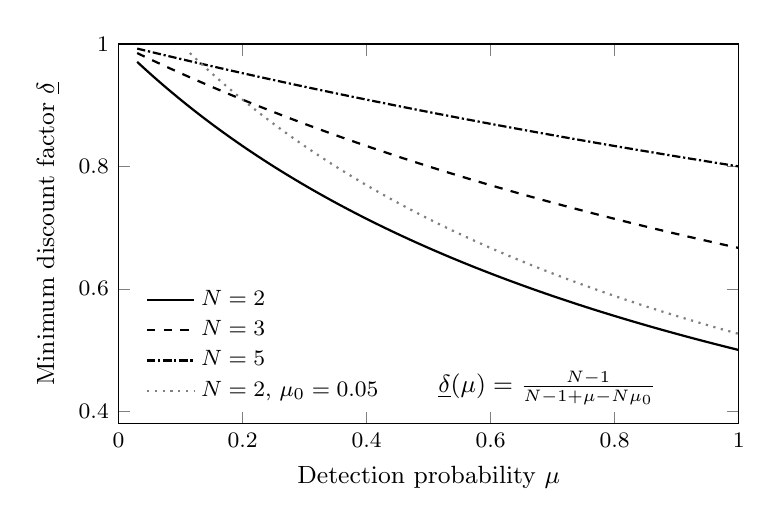
\begin{tikzpicture}
\begin{axis}[
  width=0.78\textwidth, height=6.4cm,
  xmin=0, xmax=1, ymin=0.38, ymax=1.0,
  xlabel={Detection probability $\mu$}, ylabel={Minimum discount factor $\underline{\delta}$},
  tick label style={font=\footnotesize}, label style={font=\small},
  legend pos=south west, legend style={font=\footnotesize, draw=none, fill=white},
  legend cell align=left, samples=200]
\addplot[thick, domain=0.03:1] {1/(1+x)};
\addlegendentry{$N = 2$}
\addplot[thick, dashed, domain=0.03:1] {2/(2+x)};
\addlegendentry{$N = 3$}
\addplot[thick, densely dashdotted, domain=0.03:1] {4/(4+x)};
\addlegendentry{$N = 5$}
\addplot[thick, gray, dotted, domain=0.115:1] {1/(1+x-0.1)};
\addlegendentry{$N = 2$, $\mu_0 = 0.05$}
\node[font=\small, anchor=south west] at (axis cs:0.5,0.395)
  {$\underline{\delta}(\mu) = \frac{N-1}{N-1+\mu-N\mu_0}$};
\end{axis}
\end{tikzpicture}
\caption{The minimum discount factor that sustains collusion at the monopoly price as a function of the
detection probability $\mu$, from \cref{prop:13-transparency} ($\mu_0 = 0$) and \cref{cor:13-false-alarms}
(gray dotted curve, $\mu_0 = 0.05$). With $\mu = 1$ and $\mu_0 = 0$ the threshold is $1 - \frac{1}{N}$.
False alarms shift the curve up, and with $N = 2$ collusion is impossible unless $\mu > 2\mu_0 = 0.1$.}
\label{fig:13-transparency}
\end{figure}

False alarms make collusion harder because they end collusion on the equilibrium path. This lowers the value of
colluding, and with it the loss that a deviator suffers when caught.

\begin{corollary}[False alarms]\label{cor:13-false-alarms}
Under \cref{asm:13-transparency} with $\mu_0 \in [0, \mu)$, the public grim-trigger strategy is a subgame
perfect equilibrium if and only if
\begin{equation}\label{eq:13-false-alarms}
  \delta\,(N - 1 + \mu - N\mu_0) \;\ge\; N - 1 .
\end{equation}
Collusion at $p^m$ is therefore sustainable for some $\delta < 1$ if and only if $\mu > N\mu_0$, and then the
threshold is $\frac{N-1}{N-1+\mu-N\mu_0}$. When $\mu_0 > 0$, collusion on the equilibrium path lasts a geometric
number of periods with mean $\frac{1}{\mu_0}$.
\end{corollary}

\begin{proof}
On the path a false alarm occurs with probability $\mu_0$ each period. The value of collusion solves
$V = \frac{\pi^m}{N} + \delta(1 - \mu_0)V$, so
\begin{equation*}
  V = \frac{\pi^m}{N\left(1 - \delta + \delta\mu_0\right)} .
\end{equation*}
A deviation earns at most $\pi^m$ today and $V$ tomorrow with probability $1 - \mu$. The incentive constraint is
$V \ge \pi^m + \delta(1 - \mu)V$, or $V(1 - \delta + \delta\mu) \ge \pi^m$. Substituting $V$ and multiplying by
$\frac{N(1 - \delta + \delta\mu_0)}{\pi^m}$ gives
\begin{equation*}
  1 - \delta + \delta\mu \;\ge\; N\left(1 - \delta + \delta\mu_0\right)
  \quad\Longleftrightarrow\quad
  \delta\,(N - 1 + \mu - N\mu_0) \;\ge\; N - 1 ,
\end{equation*}
which is \eqref{eq:13-false-alarms}. If $\mu > N\mu_0$, the coefficient on $\delta$ exceeds $N - 1 > 0$, and the
threshold lies below 1. If $\mu \le N\mu_0$, the left side is at most $\delta(N-1) < N - 1$ for every
$\delta < 1$, so no discount factor works. The duration statement follows from \cref{lem:13-durations} with a
per-period exit probability of $\mu_0$.
\end{proof}

\begin{remark}[Relation to Green and Porter]\label{rem:13-gp-nesting}
Set $N = 2$ and $\mu = 1$, and let $\mu_0$ be the probability of a zero-demand period in the Bertrand version of
\citet{GreenPorter1984}. A firm then always sees zero sales after a rival's undercut, and sees zero sales with
probability $\mu_0$ on the path. Condition \eqref{eq:13-false-alarms} becomes $\delta(2 - 2\mu_0) \ge 1$, or
$\delta(1 - \mu_0) \ge \frac{1}{2}$. This is the condition for collusion with permanent reversion in that model
(\cref{ch:collusion-theory}). Profits there are scaled by the probability of positive demand, and the scale
cancels from the incentive constraint. There the optimal cartel shortens punishments to limit the cost of false alarms. The
Sugar Institute lowered $\mu_0$ directly, by verifying accusations before anyone retaliated.
\end{remark}

\begin{remark}[Transparency to buyers]\label{rem:13-transparency-buyers}
Publication informs buyers as well as sellers. Better-informed buyers move faster to a price cutter, which raises
the payoff from a secret cut. Suppose a secret cut captures only a fraction $\omega \in [\frac{1}{N}, 1]$ of the
market, so a deviator earns $\omega\pi^m$. With $\mu_0 = 0$ the incentive constraint becomes
$\frac{\pi^m}{N(1-\delta)} \ge \omega\pi^m + \delta(1-\mu)\frac{\pi^m}{N(1-\delta)}$. The same algebra as in the
proof of \cref{prop:13-transparency} gives
\begin{equation*}
  \delta \;\ge\; \frac{N\omega - 1}{N\omega - 1 + \mu} .
\end{equation*}
This threshold rises with $\omega$ and falls with $\mu$. A policy that raises both $\omega$ and $\mu$ has an
ambiguous effect, so whether transparency raises or lowers prices is an empirical question.
\citet{Stigler1964} made the same point. The more buyers know about prices, the more customers a secret cut
attracts and the faster it is detected. Transparency can also help firms agree on a focal price, as the bromine
firms did when they adopted the trade-journal price after Dow War~I.
\end{remark}

\subsection{Government-assisted coordination: Danish ready-mixed concrete}\label{sec:13-concrete}

\casehead{The question}
\citet{AlbaekMollgaardOvergaard1997} study a natural experiment in transparency. Did the publication of
firm-specific transaction prices by a competition authority lower prices, as the authority intended, or did it
help firms coordinate?

\casehead{The policy}
The Danish Competition Act of 1990 stated its purpose as promoting competition ``through the largest possible
transparency of competitive conditions.'' Unlike U.S.\ and EU law, the Act rested on abuse control. It had no per
se prohibitions, and the authority intervened case by case. A \emph{per se} prohibition makes conduct illegal
without any inquiry into its effects. Under the \emph{rule of reason}, a court weighs the conduct's harm to
competition against its claimed benefits. The Competition Council interpreted the Act to mean
that suspected abuses such as oligopolistic coordination should be countered by more transparency. The premise
was that firm-specific price information lets buyers shop around and so pushes prices down.

\casehead{The product and the market}
Ready-mixed concrete is a mixture of cement, gravel, sand and water, and its strength is measured in megapascals
(MPa). A given grade is homogeneous, and different grades are imperfect substitutes. The study covers a weak grade
(10 MPa), used for foundations of single-family houses, and a strong grade (25 MPa), used for staircases.
Concrete travels in mixer lorries holding at most six cubic metres. It can stay in a lorry for only about two hours,
so it normally travels at most about twenty miles. Denmark had 115 production sites. The two main producers were
Unicon, owned by the only Danish cement producer, and 4K, and the remaining capacity belonged to independent
local firms. In 1987 the national four-firm concentration ratio was 57 percent, with Unicon at 37 percent and 4K
at 11 percent. Two years later Unicon's share reached 43 percent after it acquired the third-largest firm. Within
a radius of 20 km of a plant, many local markets were monopolies, and the average share of the largest firm was
about 70 percent. Typically fewer than five sites could serve a given customer. Pricing combined rigid, publicly
posted list prices with large confidential discounts.

\casehead{The intervention and the data}
In October 1993 the Council decided to sample invoice prices from 18 sites and publish them in its newsletter,
roughly once a quarter. The sites were in three regions, Copenhagen (7 sites), Aarhus (6) and Northern Jutland
(5). For each site and grade the Council published the list price, the average price and the average of the five
lowest prices in the first month of a quarter. Prices appeared with a lag of about three months. The data cover
the four quarters of 1994 and the first three of 1995, seven observations per site. \Cref{tab:13-albaek-timeline}
gives the timeline. The two dominant firms had almost identical list prices in each region. They set the highest
list prices and gave the largest discounts. Average discounts were 25 to 26 percent of list for 10 MPa and 27 to
31 percent for 25 MPa. Maximum discounts ranged from 25 percent in Northern Jutland to 38 percent in Aarhus.

\begin{table}[htbp]
\centering
\caption{Timeline of the Danish concrete price publication}\label{tab:13-albaek-timeline}
\small
\begin{tabular}{@{}ll@{}}
\toprule
Date & Event\\
\midrule
1990 & Competition Act adopts the transparency principle\\
October 1993 & Competition Council decides to collect and publish invoice prices\\
April 8, 1994 & January 1994 prices published\\
July 5, 1994 & April 1994 prices published\\
January to October 1994 & Weighted average price of the two grades rises 19 percent\\
April 1996 & Last publication (November 1995 prices)\\
December 1996 & Council decides to publish no more concrete prices\\
May 30, 1997 & New competition law drops the emphasis on transparency\\
\bottomrule
\end{tabular}

\smallskip
\begin{minipage}{0.8\textwidth}\footnotesize
Notes: From \citet{AlbaekMollgaardOvergaard1997}, pp.~430--433 and 440--441.
\end{minipage}
\end{table}

\casehead{The main finding}
\Cref{fig:13-albaek-f1} shows the national indices of average transaction prices for the two grades, weighted by
the firms' turnover. Prices rose sharply over the first two to three quarters of 1994. According to the Council's
reports, the weighted average increase across the two grades was 19 percent between January and October 1994.
Prices then levelled off. Over the first three quarters of 1994, consumer prices rose 1.9 percent, wholesale
prices 1.6 percent, and import prices of unprocessed raw materials 1.1 percent. An index of residential
construction costs barely moved. The unit value of all concrete produced and the unit value of cement, the main
input, show nothing like the rise in the published prices.

The comparison is a before-after design with an aggregate benchmark. Let $p_t$ be the published price index and
$p^{\mathrm{b}}_t$ a benchmark index that captures costs and general inflation. The implicit estimate of the effect
of publication is
\begin{equation}\label{eq:13-albaek-tau}
  \hat\tau = \left(\ln p_{1} - \ln p_{0}\right) - \left(\ln p^{\mathrm{b}}_{1} - \ln p^{\mathrm{b}}_{0}\right),
\end{equation}
with period 0 in January 1994 and period 1 in October 1994. With a 19 percent price rise and consumer prices as the
benchmark, $\hat\tau \approx \ln 1.19 - \ln 1.019 = 0.155$, or about 17 percent (our computation).
Interpreting $\hat\tau$ as a causal effect requires that, without publication, concrete prices would have moved
with the benchmark. The rest of the paper defends this assumption.

\begin{figure}[htbp]
\centering
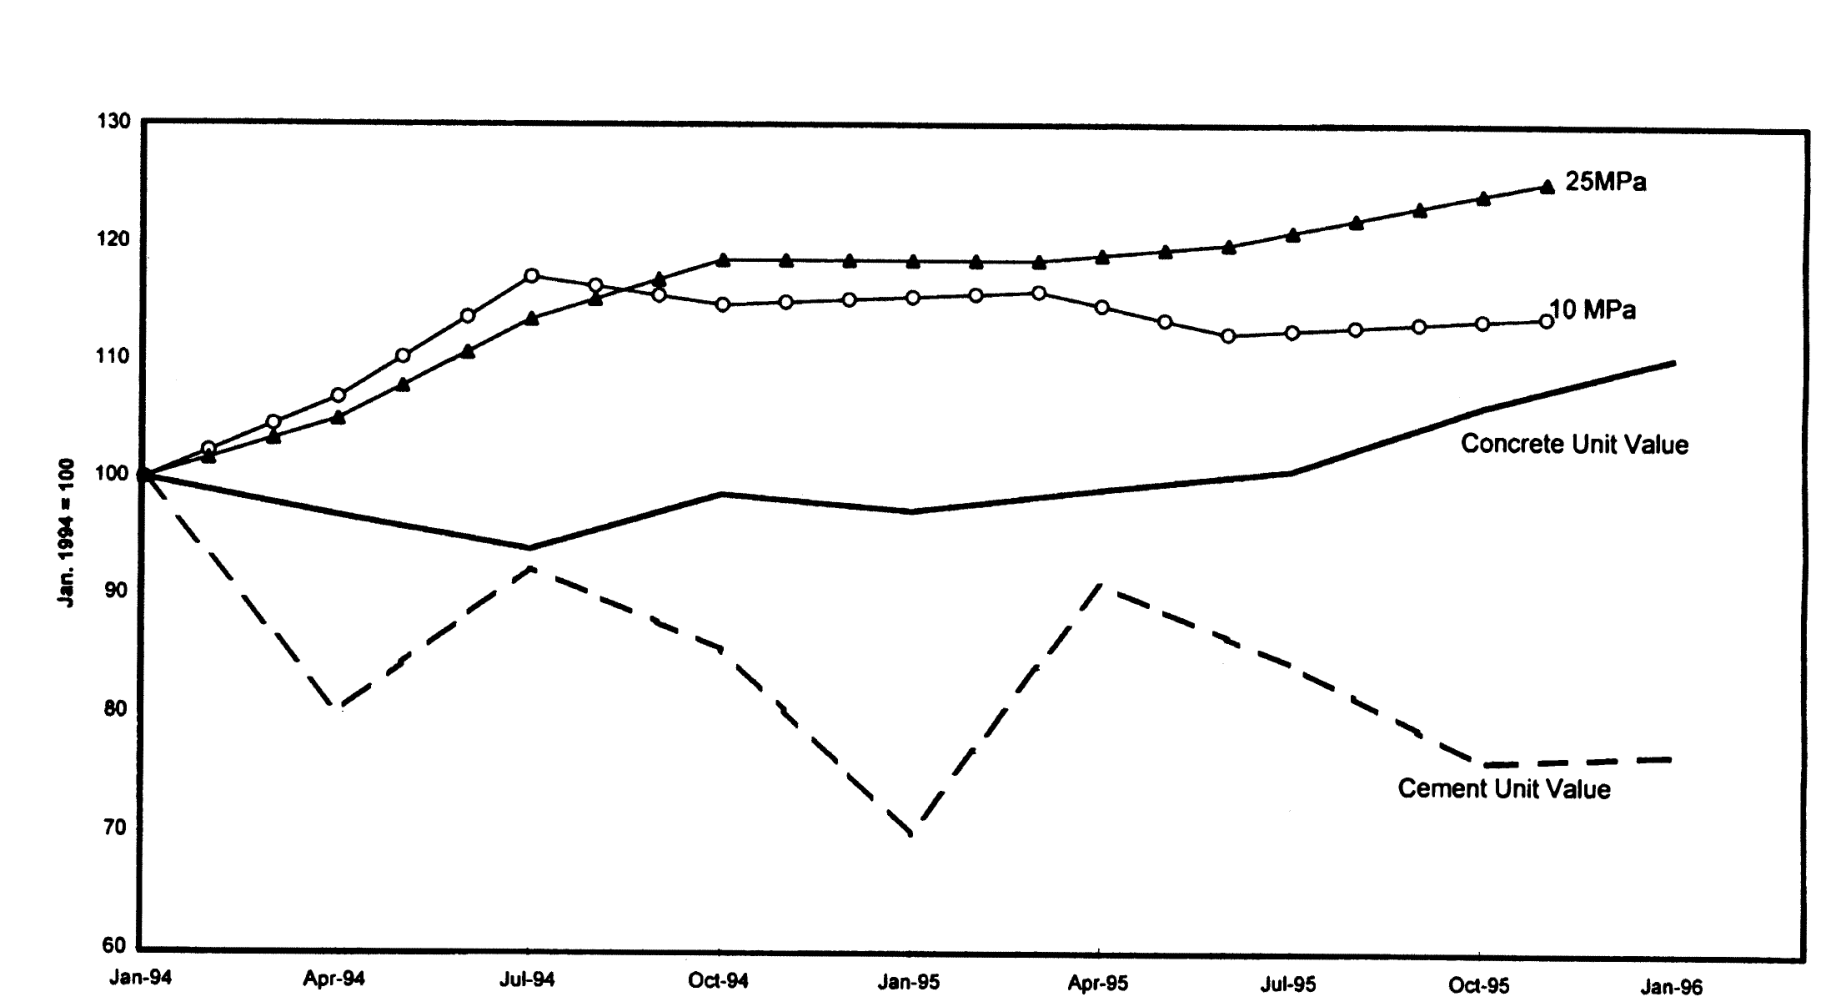
\includegraphics[width=0.88\textwidth]{figures/ch13/albaek1997_fig1.png}
\caption{National price indices for ready-mixed concrete (January 1994 = 100). The marked lines are the published
average transaction prices of 10 MPa and 25 MPa concrete. The solid line is the unit value of all concrete
produced and the dashed line the unit value of cement. Source: \citet{AlbaekMollgaardOvergaard1997}, Figure~1
(unit values from Danmarks Statistik, published prices from the Competition Council).}\label{fig:13-albaek-f1}
\end{figure}

\casehead{Ruling out competitive explanations}
In a price-setting oligopoly with capacity constraints, prices could rise because demand grew, capacity fell or
input prices rose. The authors examine each. A deep construction recession bottomed out in the summer of 1993. By
February 1994 construction employment was back at its low 1992 level. By November 1994 seasonally adjusted
employment had risen 4.4 percent and unadjusted employment 17.6 percent. Production of concrete at the end of 1993
was as low as at the trough ten years earlier. Production in 1994 was almost 20 percent above 1993 but still below
1991.

Capacity was not binding. In 1987 production was more than 50 percent above its 1994 level. Even then, capacity
utilization was about 41 percent in production and 62 percent in distribution, and productive capacity had not
fallen much since. If capacity was unchanged, utilization in 1994 was at most $\frac{62}{1.5} \approx 41$ percent in
distribution and $\frac{41}{1.5} \approx 27$ percent in production (our computation). Distribution capacity is the
number of mixer lorries, which firms could import or move between regions. Input costs did not rise either.
Wages and energy prices were flat from 1993 to 1994, and the unit value of cement fell. The cement supplier, which
owned Unicon, charged uniform delivered prices to all concrete producers.

\casehead{A closer look at Aarhus}
The authors then focus on Aarhus. Its six sampled firms carried about 70 percent of the weight in the national
indices, and price increases in the other two regions were much more moderate. Copenhagen is large, and only half
of its sites were sampled. Northern Jutland is sparsely populated, its sampled firms are local monopolies, and
its discounts were smaller at the outset. Within Aarhus the authors drop a plant on a peninsula more than 60 km
away and a Unicon plant 40 km away in Randers. The remaining four are plants of 4K and Unicon about 2 km apart in
the city, and two commonly owned local plants (Haarup and \O stjysk) 25 km and 40 km away. Together they carried
about 60 percent of the national index weight and had a combined local share close to one.

\begin{figure}[htbp]
\centering
\begin{subfigure}[b]{0.74\textwidth}\centering
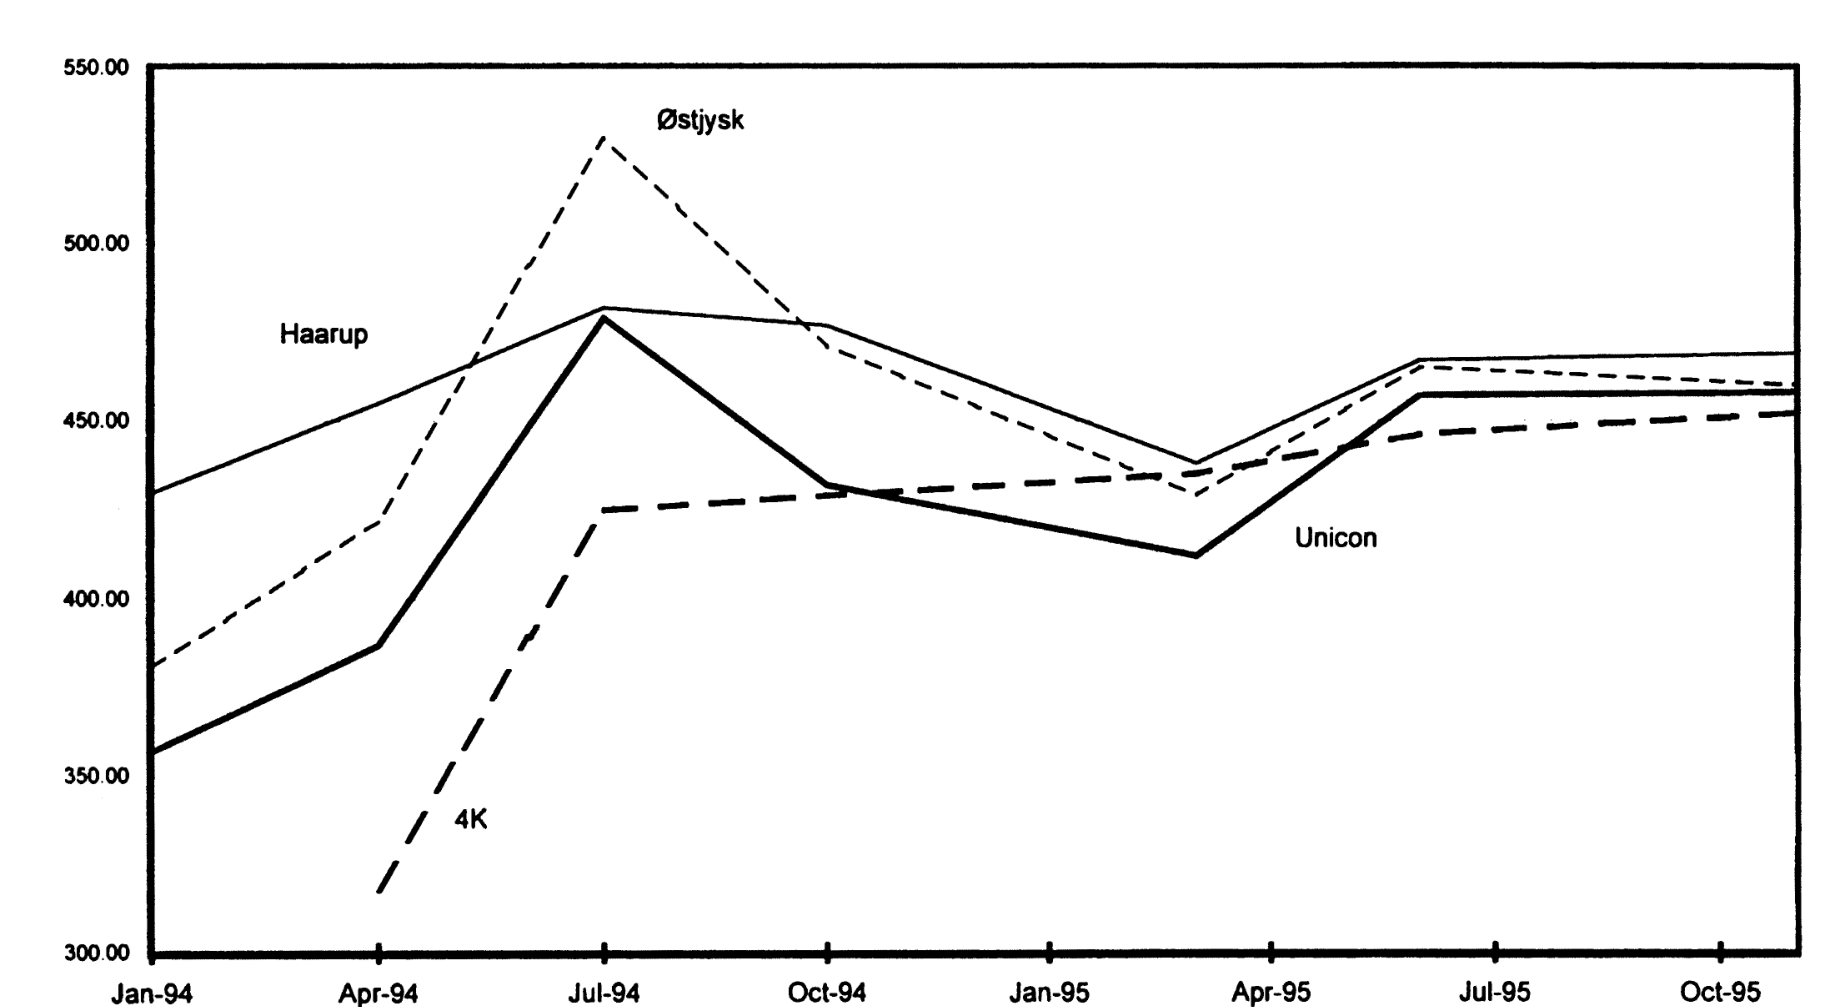
\includegraphics[width=\textwidth]{figures/ch13/albaek1997_fig2.png}
\caption{Figure 2 of the paper}
\end{subfigure}

\medskip
\begin{subfigure}[b]{0.74\textwidth}\centering
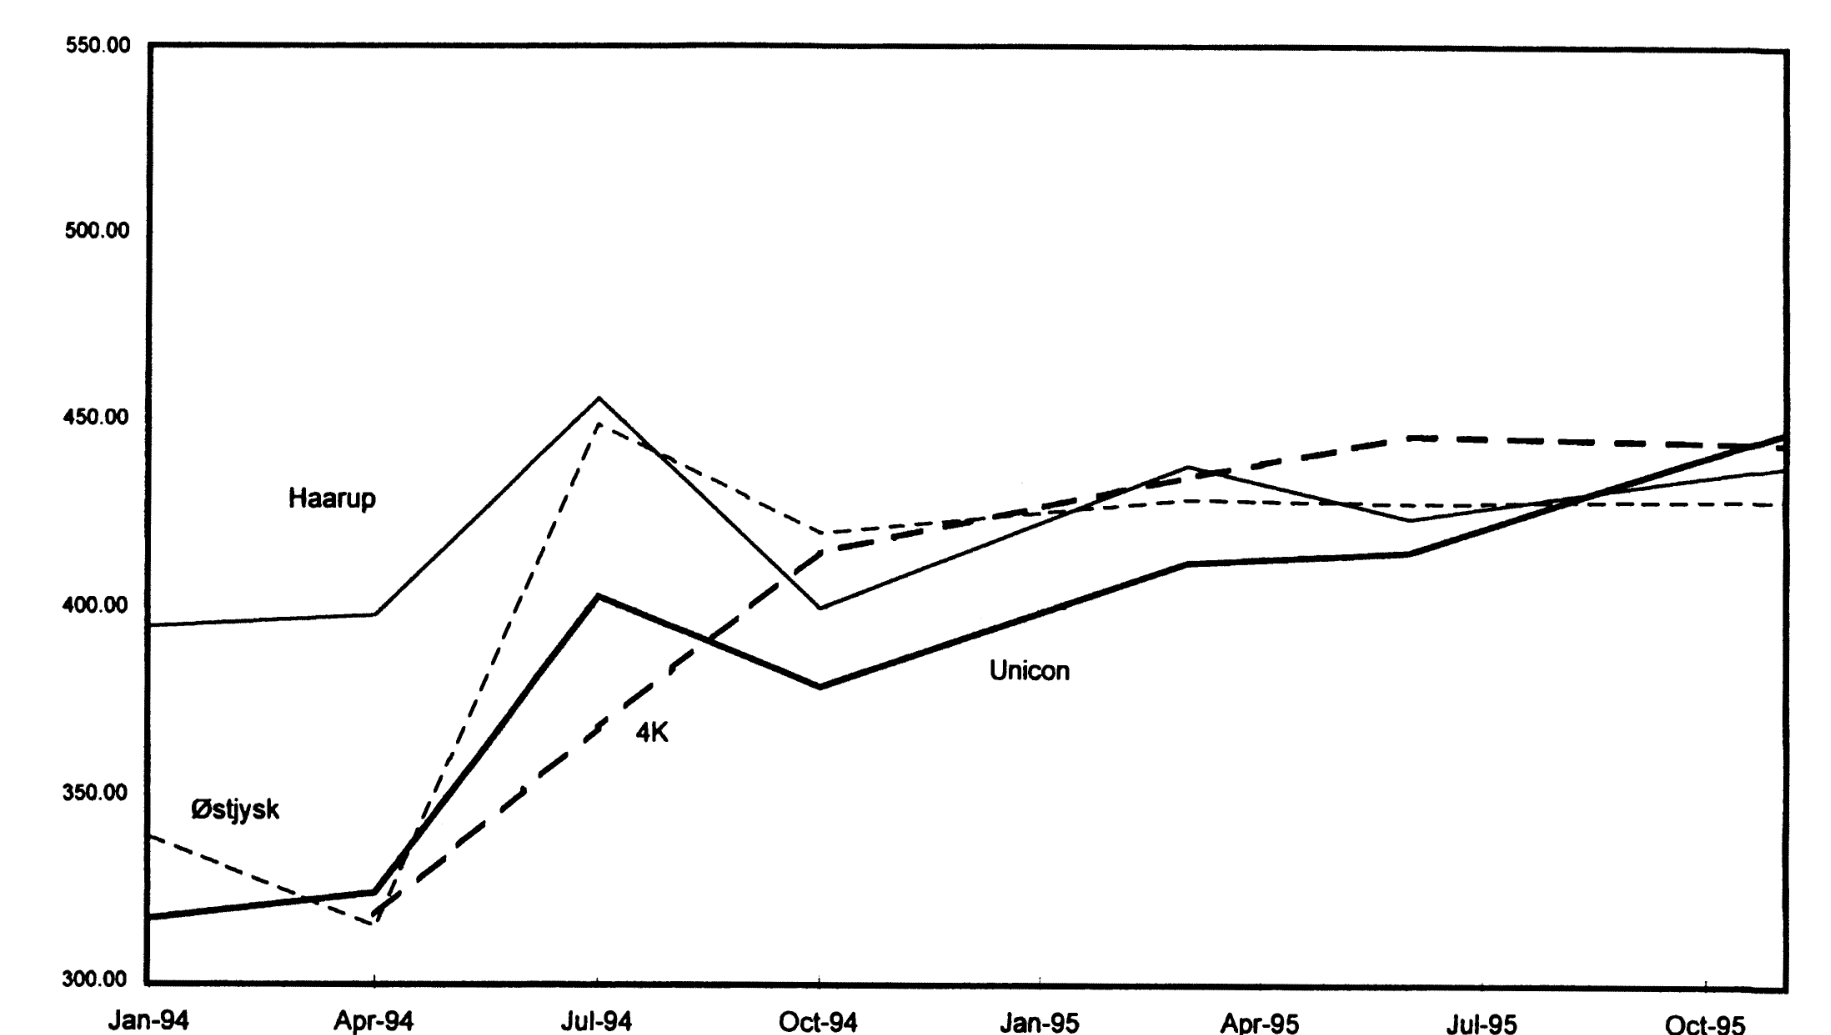
\includegraphics[width=\textwidth]{figures/ch13/albaek1997_fig3.png}
\caption{Figure 3 of the paper}
\end{subfigure}
\caption{Published 10-MPa prices of the four Aarhus plants, January 1994 to October 1995. The journal titles both
panels ``Low 10-MPa Prices in Aarhus.'' The text describes both average and low prices. Panel (b) is flat from
January to April 1994, as the text says of low prices, and lies below panel (a). We therefore read panel (a) as
average prices and panel (b) as low prices. Source: \citet{AlbaekMollgaardOvergaard1997}, Figures~2 and~3 (data from the Competition
Council).}\label{fig:13-albaek-f23}
\end{figure}

\Cref{fig:13-albaek-f23} shows the prices of these four plants. From January to April 1994, low prices were
roughly constant while average prices rose a little. From April to July 1994, prices jumped by 20 to 25 percent and
then stayed at the new level. The timing fits the flow of information. The January prices were published on April
8, 1994, so April transactions could at best partly reflect them. The April prices were published on July 5, so
by July every firm had two quarters of reliable information on rivals' formerly secret discounts. Prices also
converged. By the end of the sample, the four plants' prices varied by only 2 to 4 percent around their mean,
against up to 30 percent early in 1994. Low prices rose toward average prices, so the largest discounts
disappeared. The authors see no explanation for a 25 percent rise in tandem by two major producers 2 km apart,
other than reduced competition after secret discounts became public.

\casehead{Interpretation}
In terms of \cref{prop:13-transparency}, publication raised the detection probability $\mu$ of secret discounts.
The publication lag also mattered for \cref{rem:13-transparency-buyers}. Prices for the first month of a quarter
appeared about three months later. That told each firm what its rivals had charged, but told a buyer little about
the prices it could get today (our reading). The authors ask why a trade association had not supplied the same
information. The association said it received no price reports from members. They suggest that unverified reports
would not be credible, since a firm that gives secret discounts also gains by misreporting. The Council would also
have frowned on industry price reporting (p.~440, fn.~12). The Council itself stopped publishing at the
end of 1996. It noted that the convergence of actual and list prices since January 1994 had come entirely from a
rise in actual prices (p.~430, fn.~4). The authors also point to related evidence from U.S.\ railroad freight.
After Congress mandated the disclosure of firm-specific rail contract terms, grain rates rose.
\citet{FullerRuppelBessler1990} and \citet{SchmitzFuller1995} attribute the rise to the improved scope for
tacit collusion (p.~441).

\casehead{Limitations}
The authors list the main weaknesses. There is no control group, either regions without publication or the same
regions before publication. The Council had some data from before January 1994 but refused access. There are no
data on firms' costs or capacities, and the sample has seven quarterly observations. There is no structural model
and no standard error. One alternative they do not discuss is seasonality. The gap between adjusted and
unadjusted construction employment shows strong seasonal demand, and the jump between April and July coincides with the
building season. A seasonal rise would have reversed, however, and published prices stayed high through 1995
(our observation). Despite its limits, the paper is the cleanest evidence in this chapter that transparency can
raise prices. It also shows that a policy can harm competition through the mechanism of
\cref{prop:13-transparency}.

\subsection{Signaling through a fare-publishing system: the Airline Tariff Publishing case}\label{sec:13-atpco}

\casehead{The question}
Firms may also use an information system to communicate intentions directly. \citet{Miller2010} asks whether an
antitrust case against such communication among U.S.\ airlines changed their prices and output. The airline
industry is described in \cref{ch:airlines}.

\casehead{Setting}
The Airline Tariff Publishing (ATP) Company, owned by the airlines, is the clearinghouse for airline fares. It
collects and disseminates over 100,000 fare updates a day to airlines and to the computer reservation systems of
travel agents. Each entry contains a fare basis code, a dollar amount, a route, fare rules and footnotes, typically
first or last ticket dates. Airlines monitor the updates with sophisticated software. Travel agents can view only
one market at a time and do not see the footnote designators. In December 1992 the Department of Justice sued the
eight major domestic airlines and ATP, alleging that they used the system to communicate and to enforce price
coordination (Civil Action No.~92-2854). The alleged channels were rapid monitoring, enforcement, signaling an
intent to raise fares without shifting market shares \citep{HoltScheffman1987}, bargaining over fares and
restrictions, and linking fares across markets \citep{BernheimWhinston1990,EvansKessides1994}. In a widely cited
example, airlines punished fare cuts by America West with fare codes containing ``HP,'' America West's industry
code, and withdrew them once America West retracted its cuts. The case contrasts with an earlier and blunter
invitation to collude. In 1982 Robert Crandall, chief executive of American Airlines, telephoned Howard Putnam of
Braniff, a rival on routes out of Dallas-Fort Worth. He proposed that Braniff raise its fares by twenty percent and
promised to raise his own the next morning \citep[pp.~188--189]{AskerNocke2021}. Putnam recorded the call and turned
it over to the Department of Justice, which filed a complaint against American and Crandall. Such explicit,
private communication is easy to condemn. The ATP case concerned coded, public signals, which serve the same
purpose and are harder to prohibit (\cref{sec:12-anatomy}).

Without admitting guilt, United and US Airways settled on November 1, 1993, and the other six defendants on August
10, 1994. For ten years the airlines agreed to three restrictions. They would not use footnote indicators or fare basis
codes to convey extraneous information, or special codes linking different fares. They would not preannounce
price changes except for widely publicized sales. A facilitating practice is judged under the rule of reason \citep[p.~570]{Miller2010}, and the airlines
defended ATP as an efficient business tool. \citet{Hay2000} called a related defense ``we're naturally bad.'' It holds
that the industry's rapid monitoring alone explains supracompetitive profits, so restricting ATP would not help.
The theoretical prediction is thus ambiguous.

\casehead{Data}
Miller uses the Department of Transportation's DB1A database, a 10 percent sample of domestic tickets, from the
second quarter of 1991 to the first quarter of 1995. Fares below \$10 (presumed frequent-flyer redemptions) and
above ten times the Standard Industry Fare Level (presumed errors) are dropped, which removes less than 1 percent
of fares. The unit of observation is an airline, city-pair market and quarter. There are 411,726 such cells, with
a mean of 229 sampled tickets and a mean fare of \$209.70. Both vary widely across cells, with standard deviations
of 933.16 tickets and \$129.80, and the mean distance of a market is 1,056 miles (Table~1). The average market has
4.7 airlines, a Herfindahl index of 5,341 points and a four-firm concentration ratio of 97 percent.

\casehead{Design and estimating equation}
The identification strategy compares markets that the case should have affected with markets it should not have
affected. If ATP facilitated collusion among the defendants, the remedy should matter only where several
defendants compete. \emph{Affected} markets are city pairs served by more than two defendant airlines in every
quarter. \emph{Control} markets are city pairs where the number of major airlines is always below two. Let
$Y_{ijt}$ be tickets sold or the average fare of airline $i$ in city pair $j$ in quarter $t$. Let
$\mathit{ATP1}_t$ equal one from the second quarter of 1992, after the investigation intensified with the first
depositions in March 1992. Let $\mathit{ATP2}_t$ equal one from the first quarter of 1994, after the settlements
began. The probe itself had been announced in June 1990, and Miller dates the treatment from its intensification.
An event study finds no response of defendants' stock prices to the 1990 announcement and a significant negative
response to the intensification on March 18, 1992 (p.~574, note~9). The estimating equation is
\begin{equation}\label{eq:13-miller-did}
  Y_{ijt} = \beta_0 + \sum_{k=1}^{2}\beta_{k}^{A}\,\mathit{ATPk}_t\cdot\mathit{Aff}_j
          + \sum_{k=1}^{2}\beta_{k}\,\mathit{ATPk}_t + x_{jt}\beta_X + a_i + g_j + e_{ijt} .
\end{equation}
Here $\mathit{Aff}_j$ marks affected markets, and $a_i$ and $g_j$ are airline and city-pair fixed effects. The
controls $x_{jt}$ are the Standard Industry Fare Level, a cost measure, and the geometric means of the endpoint
states' populations and gross state products, which shift demand. Richer versions replace $\beta_k\mathit{ATPk}_t$
with quarter effects or with airline-by-quarter effects. Standard errors are clustered by city pair.

The two indicators are cumulative steps. The coefficient $\beta^{A}_1$ is the effect during the investigation, and
$\beta^{A}_1 + \beta^{A}_2$ is the effect after the settlement. A lasting effect of the remedy requires
$\beta^{A}_1 + \beta^{A}_2 \neq 0$, which Miller tests with an $F$ test. Identification rests on parallel trends.
Affected and control markets would have evolved alike absent the case, conditional on the controls. The model is
identified even with airline-by-quarter effects, because each airline serves both kinds of market before and after
the case. Affected and control markets differ in fares and distance. Miller therefore repeats the analysis with a second
control group of dominated markets, in which one airline sells over 90 percent of tickets in every quarter.

Miller also checks the results on several restricted samples (pp.~575--577). They keep flights within the
continental United States, markets with distances between 250 and 2,000 miles, and markets with stable numbers of
defendant and other airlines. One restriction counts an airline as present only if it has at least 10 sampled
tickets in the market, about 100 passengers a quarter. Another reassigns the tickets of commuter carriers to the
defendants with which they had operating agreements (p.~577, note~14). Combining all of these restrictions leaves
736 city-pair markets, the sample of columns (3) and (6) of \cref{tab:13-miller-t2}.

\begin{table}[htbp]
\centering
\caption{Quantity and price effects of the Airline Tariff Publishing case}\label{tab:13-miller-t2}
\small
\begin{tabular}{@{}lcccccc@{}}
\toprule
 & \multicolumn{3}{c}{Number of tickets} & \multicolumn{3}{c}{Average fare (dollars)}\\
\cmidrule(lr){2-4}\cmidrule(l){5-7}
 & (1) & (2) & (3) & (4) & (5) & (6)\\
\midrule
Quarter fixed effects & No & Yes & Yes & No & Yes & Yes\\
Airline $\times$ quarter effects & No & No & Yes & No & No & Yes\\
Sample restrictions & No & No & Yes & No & No & Yes\\
\addlinespace
$\mathit{ATP1}$ & 105.194 & & & 1.595 & & \\
 & (43.039) & & & (2.654) & & \\
$\mathit{ATP2}$ & 66.433 & & & $-10.746$ & & \\
 & (55.741) & & & (2.517) & & \\
$\mathit{ATP1}\times\mathit{Aff}$ & $-91.983$ & $-92.425$ & $-4.361$ & $-13.568$ & $-14.085$ & $-7.051$\\
 & (43.164) & (43.081) & (18.697) & (2.680) & (2.661) & (2.270)\\
$\mathit{ATP2}\times\mathit{Aff}$ & $-40.318$ & $-41.081$ & $-59.948$ & 12.708 & 14.619 & 2.932\\
 & (56.013) & (55.990) & (20.977) & (2.598) & (2.152) & (2.616)\\
\addlinespace
p-value, $(\mathit{ATP1} + \mathit{ATP2})\times\mathit{Aff} = 0$ & 0.08 & 0.08 & 0.05 & 0.81 & 0.86 & 0.17\\
$N$ & 328{,}921 & 328{,}921 & 10{,}934 & 328{,}921 & 328{,}921 & 10{,}934\\
City-pair markets & 4{,}825 & 4{,}825 & 736 & 4{,}825 & 4{,}825 & 736\\
$R^2$ & 0.05 & 0.05 & 0.22 & 0.04 & 0.05 & 0.34\\
\bottomrule
\end{tabular}

\smallskip
\begin{minipage}{0.95\textwidth}\footnotesize
Notes: Reproduced from \citet{Miller2010}, Table~2. The unit is an airline, market and quarter in the
10 percent ticket sample. All regressions include city-pair and airline fixed effects and the controls described
in the text. Standard errors clustered by city pair in parentheses. Columns (3) and (6) combine the sample
restrictions listed in the text, which leave 736 markets.
\end{minipage}
\end{table}

\casehead{Results}
\Cref{tab:13-miller-t2} reproduces the main estimates. Tickets rose in affected markets after the case, but they
rose more in control markets. In column (1) the relative change after the settlement is
$-91.983 - 40.318 = -132.3$ sampled tickets per airline, market and quarter, significant at the 8 percent level.
Multiplying by 10 to undo the sampling gives about 1,300 tickets, the ``over 1,000 tickets per quarter'' in the
text (our reconstruction). Column (3) gives $10 \times (4.361 + 59.948) = 643$, matching the reported
postsettlement decline of 640 tickets, significant at the 5 percent level. Lower relative traffic contradicts a
lasting increase in competition and fits the airlines' claim that the restrictions made travel planning harder.

Fares fell and then recovered. In column (4), affected-market fares fell \$13.57 relative to control markets
during the investigation and rose \$12.71 after the settlement. The net effect of $-\$0.86$ is insignificant
($p = 0.81$). With the average fare near \$210, the initial fall is about 6.5 percent (our computation). In logs,
the two coefficients are $-0.088$ and $0.035$, both significant. The pattern holds across the fare distribution.
With quarter effects, the investigation lowered the 10th percentile, median and 90th percentile fares by \$9.08,
\$10.98 and \$28.93, and the settlement raised them by \$9.51, \$14.76 and \$21.24 (Table~3). Price dispersion
therefore fell and then rose, and only the 90th percentile shows a net decline, significant at the 10 percent
level.

\begin{figure}[htbp]
\centering
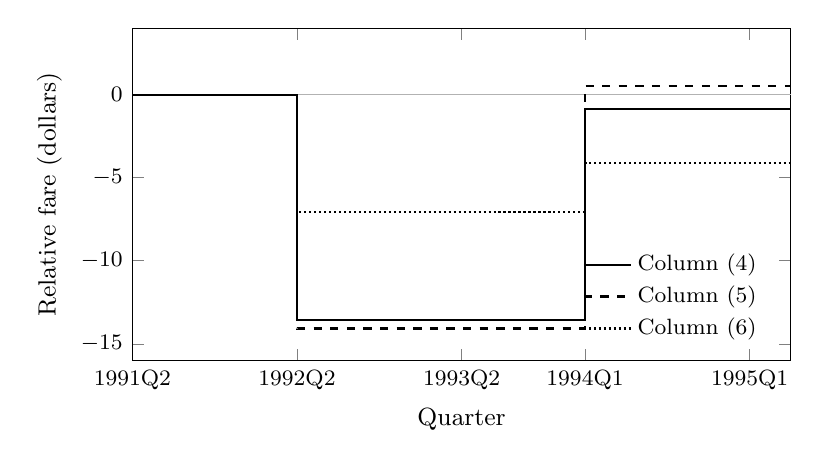
\begin{tikzpicture}
\begin{axis}[
  width=0.82\textwidth, height=5.8cm,
  xmin=1991.25, xmax=1995.25, ymin=-16, ymax=4,
  xlabel={Quarter}, ylabel={Relative fare (dollars)},
  xtick={1991.25,1992.25,1993.25,1994.0,1995.0},
  xticklabels={1991Q2,1992Q2,1993Q2,1994Q1,1995Q1},
  tick label style={font=\footnotesize}, label style={font=\small},
  legend pos=south east, legend style={font=\footnotesize, draw=none, fill=none}, legend cell align=left]
\draw[gray!60] (axis cs:1991.25,0) -- (axis cs:1995.25,0);
\addplot[thick, const plot] coordinates {(1991.25,0) (1992.25,-13.568) (1994.0,-0.860) (1995.25,-0.860)};
\addlegendentry{Column (4)}
\addplot[thick, dashed, const plot] coordinates {(1991.25,0) (1992.25,-14.085) (1994.0,0.534) (1995.25,0.534)};
\addlegendentry{Column (5)}
\addplot[thick, densely dotted, const plot] coordinates {(1991.25,0) (1992.25,-7.051) (1994.0,-4.119) (1995.25,-4.119)};
\addlegendentry{Column (6)}
\end{axis}
\end{tikzpicture}
\caption{Average fares in affected markets relative to control markets implied by
\citet{Miller2010}, Table~2. The path is 0 before the second quarter of 1992, $\beta^{A}_1$ during the
investigation, and $\beta^{A}_1 + \beta^{A}_2$ from the first quarter of 1994. Our construction from the reported
coefficients.}\label{fig:13-miller-path}
\end{figure}

\Cref{fig:13-miller-path} plots the implied fare paths. Two further results support the reading of a temporary
effect. Separate regressions for defendants and other airlines show that the fall and rise in fares came from the
defendants, whose relative fares fell \$8.71 and then rose \$10.49 (Table~4). Their relative ticket sales rose
during the investigation, while other airlines lost traffic. The defendants' fare cuts mostly shifted passengers
from other carriers. Miller also re-estimates the multimarket-contact regression of \citet{EvansKessides1994}:
\begin{equation}\label{eq:13-miller-mmc}
  \ln \mathit{Price}_{ijt} = x_{ijt}\beta_X + \beta_Z Z_{jt} + \sum_{k=1}^{2}\beta_{Zk}\,\mathit{ATPk}_t\cdot Z_{jt}
    + a_i + g_j + \tau_t + e_{ijt} .
\end{equation}
Here $Z_{jt}$ is the average number of routes that the airlines serving market $j$ have in common, divided by
1,000. The controls $x_{ijt}$ include the airline's route and airport shares and the route Herfindahl index. In the
Evans-Kessides sample, the contact coefficient is 0.269 (0.043). It falls by 0.104 (0.030) during the
investigation and rises by 0.107 (0.033) after the settlement, with a p-value of 0.96 for no net change
(Table~5). In this sample the contact effect weakened while the case was active, to $0.269 - 0.104 = 0.165$, or
about three fifths of its initial value. After the settlement it rose to $0.165 + 0.107 = 0.272$, close to its
initial value. The p-value concerns the net change,
so it says nothing about whether the coefficient of 0.165 differs from zero. In the two larger samples the
interaction largely offsets the baseline coefficient, $0.016 - 0.014$ and $0.035 - 0.025$, and Miller reports that
contact was then an insignificant predictor of prices (p.~582). Finally, the hub premium,
which should have risen if collusion in contested markets broke down, fell by about 8 percent during the
investigation and by another 13 percent after the settlement.

\casehead{Interpretation and critiques}
The defendants lowered fares under the scrutiny of the investigation and raised them once the settlement was in
place. The settlement left the system largely intact, including the rapid fare monitoring that lets airlines
detect and match fare cuts. In terms of \cref{prop:13-transparency}, the remedy removed some signaling devices but
left the detection probability $\mu$ high. The business press described weekend fare changes as a near substitute
for the forbidden preannouncements. American Airlines was later accused of violating the decree and accepted a
new seven-year decree in 2004. Alternatively, the airlines may never have used ATP as alleged.
\citet{Borenstein2004} reports relative price increases after the settlement on 387 routes likely to be affected,
consistent with Miller.

The design has weaknesses that Miller discusses. Group membership depends on entry and exit, which are outcomes.
She treats it as predetermined over four years and drops markets whose group changes. Southwest's entry was more
frequent in affected markets, and the results survive dropping markets that Southwest entered or left. Affected
and control markets differ in fares, distances and traffic, which weakens parallel trends, so she repeats the
analysis with dominated markets as controls. The timing of treatment is also uncertain. The probe was announced in
June 1990, the suit filed in December 1992, and the settlements signed in 1993 and 1994. The paper does not report
pre-trends, so the identifying assumption cannot be checked directly (our observation). The case connects to the
retrospective methods of \cref{sec:13-enforcement}. Miller reads the time pattern of fares as a sign that the
settlement failed because of its limited scope, and she rejects the reading that the industry was already
competitive (p.~570). She also warns that a weak settlement can be empirically indistinguishable from one applied
to an already competitive industry (p.~573). The pattern is consistent with a remedy that removed signaling devices
while leaving rapid fare monitoring and other coordination channels intact. The design does not separately identify
these channels.

\subsection{Rules among nonprofits: the Overlap group and financial aid}\label{sec:13-overlap}

\casehead{The question}
Can an agreement on rules among nonprofit institutions raise prices? \citet{CarltonBambergerEpstein1995} study the
antitrust case against the Overlap group of universities. They ask whether the schools' agreement on financial aid
raised the average price that students paid. They also ask how antitrust law should treat collective action by
nonprofits. The study grew out of work by Lexecon for MIT, and Carlton testified as MIT's expert witness, as the
paper discloses.

\casehead{The agreement}
In the 1950s the Ivy League schools met to stop bidding for star athletes. They agreed that no athlete would
receive aid beyond financial need, and soon applied the same idea to star students. By the 1970s the Overlap
meetings included the eight Ivy League schools, MIT and 14 other selective colleges, 23 schools in all. Their
combined undergraduate enrollment of about 60,000 was less than one percent of the national total.
\Cref{fig:13-cbe-aid} shows the accounting. Let $\bar p$ be the gross charge for tuition, room, board and fees. A
student covers it with grants $G$, self help $H$ (loans and jobs) and a family contribution $F$. In this subsection
$G$, $H$ and $F$ are local symbols for these three sources, not distribution functions:
\begin{equation}\label{eq:13-cbe-accounting}
  \bar p = G + H + F, \qquad \text{aid package} = G + H, \qquad \text{payment to the school} = H + F = \bar p - G .
\end{equation}
The Overlap schools agreed to give aid only on the basis of need and to use a common method to define need. They
also met to discuss individual students admitted by more than one school. A printout of commonly admitted students
listed each school's proposed family contribution. When proposals differed by more than several hundred dollars,
the schools discussed them and usually agreed on a common figure. Disagreements arose for 10 to 20 percent of the
commonly admitted students who applied for aid. Regardless of which Overlap school admitted a student, the family
contribution $F$ was the same. Some schools also agreed on the split of the aid package between $H$ and $G$.

\begin{figure}[htbp]
\centering
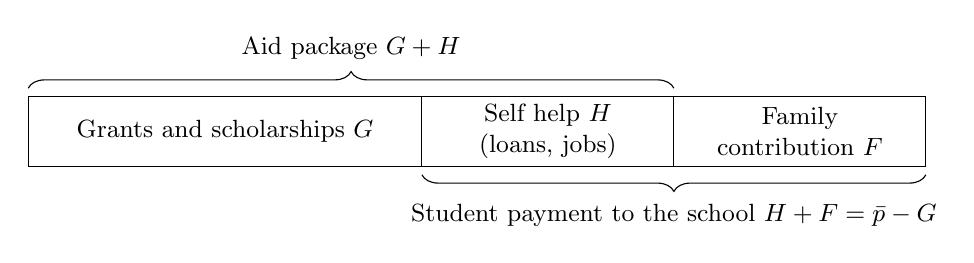
\begin{tikzpicture}[font=\small]
\draw (0,0) rectangle (5,0.9) node[pos=0.5, align=center] {Grants and scholarships $G$};
\draw (5,0) rectangle (8.2,0.9) node[pos=0.5, align=center] {Self help $H$\\(loans, jobs)};
\draw (8.2,0) rectangle (11.4,0.9) node[pos=0.5, align=center] {Family\\contribution $F$};
\draw[decorate, decoration={brace, amplitude=6pt}] (0,1.0) -- (8.2,1.0)
  node[midway, above=7pt] {Aid package $G + H$};
\draw[decorate, decoration={brace, amplitude=6pt, mirror}] (5,-0.1) -- (11.4,-0.1)
  node[midway, below=7pt] {Student payment to the school $H + F = \bar p - G$};
\end{tikzpicture}
\caption{The components of the gross charge $\bar p$ for a student receiving aid. The Overlap schools agreed on the
family contribution $F$ of commonly admitted aid applicants. Redrawn from \citet{CarltonBambergerEpstein1995},
Figure~1.}\label{fig:13-cbe-aid}
\end{figure}

The schools justified the agreement as a way to concentrate scarce aid on needy students, supporting need-blind
admission with a guarantee of full aid for every admitted student. Few schools outside Overlap made both
commitments. Federal aid policy had the same logic, since federal money generally goes only to needy students.

\casehead{The case}
In 1991 the Antitrust Division sued MIT and the eight Ivy League schools under Section~1 of the Sherman Act. It
called the agreement ``garden variety price fixing'' on the number and size of discounts from list price. By
limiting discounts, it claimed, the schools raised the prices paid by meritorious high-income students and the
average price paid by all. There was no allegation that enrollment fell, and enrollment growth at Overlap and
non-Overlap private schools was similar in 1984--1990. The Government asked for per se condemnation. The Ivy League
schools signed a consent decree, and MIT went to trial. In July 1992 Congress passed the Higher Education Act
of 1992. It gave prospective antitrust immunity to much Overlap-type conduct but not to discussions of individual
students. In September 1992 the District Court found MIT guilty of price fixing. In September 1993 the Court of
Appeals overturned the
verdict and ordered a full rule-of-reason analysis that weighed the social benefits claimed by MIT. In December 1993
the Government settled. MIT and other schools could agree not to give merit aid, use common principles to assess
need, pool student information and audit departures, but could not discuss individual awards.

\casehead{Theory}
The authors argue that the Government's claim that average prices must rise is wrong as a matter of theory for
nonprofits. A university's objective has many attributes, including the quality of education, the welfare of
students, faculty and administrators, research, innovation and donors' preferences. At MIT, student charges covered
only about half the full cost of education. Schools erect barriers to trade that a profit maximizer would not. They
do not sell admission, and the authors suspect that Harvard or MIT could profitably auction its last five places.
Raising the average price would raise revenue for valued uses but would harm students, who are part of the
objective. The authors also ask why schools colluding to raise revenue would target needy students rather than
rich ones, and why they would keep need-blind admission. These facts raise doubts but cannot rule out a price
effect, so the question is empirical.

The accounting identity \eqref{eq:13-cbe-accounting} shows what the data can test. Let $n$ students attend a
school and let $G_s$ be student $s$'s institutional grant. Average net revenue per student is
\begin{equation}\label{eq:13-cbe-avg}
  p = \bar p - \frac{1}{n}\sum_{s=1}^{n} G_s .
\end{equation}
The Government's theory implies that Overlap lowered total grants $\sum_s G_s$ and so raised $p$. The schools'
theory implies that Overlap reallocated grants from merit to need, changing the distribution of $G_s$ without
changing their sum. Average net price $p$ discriminates between the two theories. It is silent on how the
agreement redistributed aid.

\casehead{Data}
A before-and-after comparison is infeasible. Overlap had met for over 30 years, and it stopped after the 1991--1992
academic year, leaving only two years of data contaminated by the lawsuit. The authors therefore compare schools.
The 23 Overlap schools fall into five 1987 Carnegie classifications, and annual data for 1984--1990 cover about 225
private and public schools in these classes. The dependent variable is the real average price per student. It equals gross
tuition plus room and board plus mandatory fees minus the average institutionally administered grant per student,
deflated to 1990 dollars by the consumer price index. Institutional grants are the school's own money plus small
federal SEOG grants of about \$50 per undergraduate. For the 162 private schools in the pooled sample, the average
net price is \$12,366 with a standard deviation of \$2,420 (Table~4).

The regressors in their Table~2 are an Ivy-plus-MIT Overlap dummy $\mathit{IVY}$ and an other-Overlap dummy
$\mathit{NONIVY}$. Carnegie dummies are $\mathit{RSRCH1}$, $\mathit{RSRCH2}$, $\mathit{DOCTOR1}$ and
$\mathit{DOCTOR2}$, with Liberal Arts~I omitted. Quality is measured by the percent of applicants accepted
($\mathit{PCTACC}$), the percent scoring above 700 on the verbal or mathematics SAT ($\mathit{SAT}$) and the
percent completing a degree ($\mathit{COMPDEG}$). Financial capacity is measured by real endowment per
full-time-equivalent student in thousands ($\mathit{ENDOW}$) and by the percent of students not receiving
need-based aid ($\mathit{PCTNOAID}$, a wealth proxy). Real state per capita disposable income ($\mathit{YDPC}$)
proxies both income and costs. Further dummies mark non-religious schools ($\mathit{NONRELIG}$), public schools
($\mathit{PUBLIC}$) and missing fee data ($\mathit{FEEMISS}$).

\casehead{Estimating equations}
For school $i$ in year $t$, the annual cross-section model is
\begin{equation}\label{eq:13-cbe-annual}
  p_{it} = x_{it}\beta_t + e_{it},
\end{equation}
estimated separately for each year by least squares. Here $i$ indexes schools, a local use. Because the regressors
change slowly within a school, a pooled regression essentially uses cross-school variation. The authors
therefore also estimate a school-average model. Let $N_i$ be the number of years with data for school $i$ and let
$d_{it} = \frac{1}{N_i}$ for those years. Averaging \eqref{eq:13-cbe-annual} with a common $\beta$ gives
\begin{equation}\label{eq:13-cbe-average}
  \bar p_i = \sum_t d_{it}p_{it} = \Big(\sum_t d_{it}x_{it}\Big)\beta + \sum_t d_{it}e_{it} .
\end{equation}
If the $e_{it}$ are uncorrelated over time with common variance $\sigma^2$, the averaged error has variance
$\Var\big(\sum_t d_{it}e_{it}\big) = \frac{\sigma^2}{N_i}$. Multiplying \eqref{eq:13-cbe-average} by
$\sqrt{N_i}$ makes the error homoskedastic, and least squares on the transformed equation is generalized least
squares. This is why the authors weight by $\sqrt{N_i}$ (WP p.~19, fn.~22). They also report White standard errors,
which are similar.

\begin{table}[htbp]
\centering
\caption{Determinants of the average net price per student at private colleges}\label{tab:13-cbe-t6}
\small
\begin{tabular}{@{}lcc@{\hspace{2.2em}}lcc@{}}
\toprule
\multicolumn{6}{@{}l}{\textit{Panel A. School averages, 1984--1990, weighted by $\sqrt{N_i}$ (Table 6)}}\\
\midrule
Variable & Coef. & (s.e.) & Variable & Coef. & (s.e.)\\
\midrule
Intercept & 2299.47 & (2429.07) & $\mathit{PCTACC}$ & $-27.89$ & (11.97)\\
$\mathit{IVY}$ & $-322.42$ & (678.72) & $\mathit{PCTNOAID}$ & 43.58 & (9.44)\\
$\mathit{NONIVY}$ & 130.37 & (463.81) & $\mathit{SAT}$ & 2.31 & (11.16)\\
$\mathit{RSRCH1}$ & 1042.21 & (435.09) & $\mathit{YDPC}$ & 0.36 & (0.07)\\
$\mathit{RSRCH2}$ & 1062.57 & (514.05) & $\mathit{COMPDEG}$ & 45.68 & (16.64)\\
$\mathit{DOCTOR1}$ & 545.66 & (551.02) & $\mathit{NONRELIG}$ & 1343.18 & (250.19)\\
$\mathit{DOCTOR2}$ & $-1143.27$ & (493.21) & $\mathit{ENDOW}$ & $-5.95$ & (3.77)\\
$\mathit{FEEMISS}$ & $-540.82$ & (294.78) & Observations & \multicolumn{2}{c}{162}\\
\midrule
\multicolumn{6}{@{}l}{\textit{Panel B. Overlap coefficients in the annual regressions (Table 5)}}\\
\midrule
 & 1984 & 1985 & 1986 & 1987 & 1989\\
\midrule
$\mathit{IVY}$ & 271.84 & 21.92 & 4.14 & 16.87 & $-918.91$\\
 & (714.52) & (788.16) & (762.04) & (882.56) & (1079.05)\\
$\mathit{NONIVY}$ & 120.53 & 172.84 & 173.84 & 688.30 & 161.56\\
 & (468.39) & (529.46) & (517.53) & (658.66) & (650.61)\\
$N$ & 130 & 137 & 136 & 106 & 105\\
\bottomrule
\end{tabular}

\smallskip
\begin{minipage}{0.95\textwidth}\footnotesize
Notes: Reproduced from \citet{CarltonBambergerEpstein1995}, NBER working-paper version, Tables~5 and~6.
Dependent variable: real gross tuition, room, board and mandatory fees minus the average
institutional grant per student, in 1990 dollars. Standard errors in parentheses. Panel B also has a 1990
column, with $\mathit{IVY}$ $-2.22$ (1681.46), $\mathit{NONIVY}$ 422.67 (1092.78) and $N = 53$. No Ivy Overlap
school reported complete data for 1988.
\end{minipage}
\end{table}

\casehead{Results}
\Cref{tab:13-cbe-t6} reproduces the results for private schools. In no annual regression is either Overlap
coefficient positive and significant. In the pooled average regression, $\mathit{IVY}$ is $-322$ dollars with a
standard error of 679, and $\mathit{NONIVY}$ is 130 dollars with a standard error of 464. If anything, Overlap
schools charged less, though not significantly so. With gross charges as the dependent variable, the Overlap
coefficient is $-376$ dollars and insignificant (fn.~24). The authors also display the fit school by school
(their Figures~2 and~3). Equation \eqref{eq:13-cbe-average} overpredicts the average price of four of the seven
Ivy-plus-MIT schools with data and underpredicts it for the other three. Their residuals are small and average
close to zero. The other coefficients are sensible. Schools with richer
students charge more, and non-religious schools charge about \$1,500 more than religious ones in the annual
regressions.
Including public schools gives about 225 schools and a significant public-school effect of about $-\$8{,}400$.

The quality premium is modest. Compare a selective school ($\mathit{PCTACC} = 25$, $\mathit{COMPDEG} = 80$) with a
less selective one ($\mathit{PCTACC} = 75$, $\mathit{COMPDEG} = 40$). The predicted difference is
\begin{equation*}
  -27.89\,(25 - 75) + 45.68\,(80 - 40) = 1{,}394.5 + 1{,}827.2 = 3{,}222 \text{ dollars}
\end{equation*}
(our computation), the ``roughly \$3000'' of the text and about a quarter of the average price. The authors compare
it with the return to an elite education. \citet{JamesEtAl1989} find that graduates of elite schools earn 3 to 5
percent more. With a base income of \$50,000, a 5 percent premium and a 10 percent real interest rate, the premium
is worth about $\frac{0.05 \times 50{,}000}{0.10} = 25{,}000$ dollars as a perpetuity.

\casehead{Robustness}
The finding survives several checks. Generalized least squares on the panel with equicorrelated errors within a
school gives a correlation of about 0.8 and results like those in \cref{tab:13-cbe-t6}. A random-effects model
cannot be distinguished from a fixed-effects model by a \citet{Hausman1978} test. The fixed-effects model cannot
identify the Overlap effect, but its other coefficients match. Results are unchanged with public schools
included, with suspect duplicate observations dropped, with quadratic terms in $\mathit{PCTACC}$,
$\mathit{COMPDEG}$ and $\mathit{ENDOW}$, and with logs. Dropping the wealth variable, which is the regressor most
likely to be endogenous, or lagging it, leaves the Overlap coefficients unchanged. To address the endogeneity of
Overlap membership itself, the authors estimate the model on non-Overlap schools only and test whether it fits the
excluded schools. An $F$ test never rejects, and the model predicts the Overlap schools' average prices well.

\casehead{The case for collective action}
The authors argue that without Overlap, competition for star students would have diverted aid from needy to
meritorious students. Merit aid was growing as a share of institutional aid. Across 72 schools, the ratio of merit
aid to need aid rose from 0.134 in 1984 to 0.180 in 1989, and among Liberal Arts~I colleges from 0.076 to 0.131
(Table~7). To test whether Overlap raised access, they regress the log odds of the black or Hispanic share of
students on the same variables (Table~8). One regressor is added, the state's minority share of the college-age
population. For black
students the Overlap coefficient is 0.451 (0.172). Splitting it, $\mathit{IVY}$ is 0.396 (0.268) and
$\mathit{NONIVY}$ 0.478 (0.198). For Hispanic students the coefficient is 0.183 (0.146), with $\mathit{IVY}$ 0.025
(0.227) and $\mathit{NONIVY}$ 0.258 (0.167). A log-odds effect of 0.451 raises a 3 percent share to
$\frac{0.0309 \times e^{0.451}}{1 + 0.0309 \times e^{0.451}} = 4.6$ percent (our computation), close to the
authors' ``about five rather than about three percent.'' They note that Overlap schools may simply have recruited
black students harder.

The Court of Appeals distinguished the case from \textit{National Society of Professional Engineers},
where the Supreme Court struck down a quality-motivated bidding restriction by an association of profit-maximizing
members. It noted ``the absence of any finding of adverse effects such as higher price or lower output'' and that
the agreement was not intended to raise revenue. The authors support this reasoning. Institutions granted
501(c)(3) status pursue social goals that competition among profit maximizers does not achieve. If such goals
could never justify collective action, no collective action by nonprofits would be legal.

\casehead{Critiques}
Identification is by selection on observables in a cross-section. Overlap membership is not random, and
the Ivy-plus-MIT coefficient rests on seven schools with data (Dartmouth and Cornell are missing), all at the
extremes of selectivity and wealth. Some controls may themselves respond to Overlap. The share of students not
receiving need-based aid, $\mathit{PCTNOAID}$, depends on aid policy, and conditioning on it can absorb part of the
effect being measured (our observation). The test concerns the mean of the price distribution, while the
schools' own account implies a change in its shape, a transfer from meritorious high-income students to others.
The authors' conclusion says exactly this. Finally, the test has limited power. The 95 percent confidence interval
for $\mathit{IVY}$ is
\begin{equation*}
  -322.42 \pm 1.96 \times 678.72 = [-1{,}653,\; 1{,}008] \text{ dollars}
\end{equation*}
(our computation). The data cannot rule out an Overlap price effect of about \$1,000, or 8 percent of the average
price. A finding of no significant effect is a statement about precision. The contrast with Danish concrete is
instructive. There the outcome moved by 20 percent within two quarters, and even a crude design could detect it.

\subsection{What the information cases show}\label{sec:13-information-lessons}

The three cases fit the logic of \cref{prop:13-transparency} and \cref{rem:13-transparency-buyers}. Publishing
past transaction prices raised the detection probability of secret discounts more than it informed buyers, and
concrete prices rose. The airline remedy removed signaling codes but left rapid monitoring in place. Fares
returned to their earlier relative level, which is consistent with coordination through the channels that remained,
although the design cannot separate those channels. The Overlap agreement concerned the allocation of aid among students. It
had no detectable effect on average prices, and its likely effects were distributional. Together with the Sugar
Institute and bromine, these cases show that information is a strategic variable. Firms invest in detection,
outside bodies can supply it, and the effect of any change depends on who learns what and how fast.
